% Define all the needed variable like it is shown in the var.tex.example
% (Just copy the var.tex.example file and remove the ".example" from the filename.)
% specify the relative path from the main file to the folder that contains the template repo
\newcommand{\templatePath}{template}

% define some information about this summary
\newcommand{\summaryTitle}{Quantum Mechanics}
\newcommand{\summarySubTitle}{FS24 ETHZ}
\newcommand{\summaryAuthor}{Juri Pfammatter, Daniel Schweizer and Tobias Meier}
\newcommand{\repoURL}{https://github.com/MeierTobias/eth-quantum-mechanics}
\newcommand{\summaryInfo}{This PDF, the source code as well as the disclaimer can be found in the GitHub repository \url{\repoURL}.}
\newcommand{\imagePath}{./images/}

% layout options
\newcommand{\orientationmode}{portrait} % landscape or portrait
\newcommand{\papersize}{a3paper} % a4paper or a3paper
\newcommand{\fontheight}{10pt}

% additional conditions
\newcommand{\includeexamples}{1} % 0 = don't show examples, 1 = show examples

\documentclass[\fontheight]{extarticle}

% load the template headers
\input{\templatePath/summary_headers.tex} % ChkTex 27

\begin{document}
\begin{multicols*}{3}
    
    % create the title section
    \input{\templatePath/summary_title.tex} % ChkTex 27
    \section{Introduction}

\subsection{Schrödinger Equation for Matter}
\begin{align*}
               &  & i\hbar \frac{\partial \Psi(\mathbf{r},t)}{\partial t} & = \underbrace{- \frac{\hbar^2}{2m} \nabla^2 \Psi(\mathbf{r},t)}_{E_{kin}} + \underbrace{V(\mathbf{r},t)\Psi(\mathbf{r},t)}_{E_{pot}} \\
    \text{1D:} &  & i\hbar \frac{\partial \Psi(x,t)}{\partial t}          & = \underbrace{- \frac{\hbar^2}{2m} \frac{\partial^2 \Psi(x,t)}{\partial x^2}}_{E_{kin}} + \underbrace{V(x,t)\Psi(x,t)}_{E_{pot}}
\end{align*}

\renewcommand{\arraystretch}{1.3}
\setlength\tabcolsep{6pt} % default value: 6pt
\begin{tabularx}{\linewidth}{@{}ll@{}}
    $\hbar = \frac{h}{2\pi}$ & $h$: Planck constant          \\
    $m,t,x$                  & Mass, time, position          \\
    $V(x,t)$                 & Potential energy function     \\
    $\Psi$                   & Complex particle wavefunction \\
                             & (``probability amplitude'')     \\
\end{tabularx}
\renewcommand{\arraystretch}{1}
\setlength\tabcolsep{6pt} % default value: 6pt
\subsection{QM and Classical Physics}
\subsubsection{Planck}
When describing black body radiation with classical physics, the problem of \textit{infinite radiation at
    high frequencies at any temperature} occurs, because each of the infinite modes need a small amount of energy.
Classical physics predicts a radiation power per unit area and frequency 
\begin{equation*}
    P \propto k_B T \nu^2
\end{equation*}
because the number of modes, each with energy $k_B T$ (measure of average thermal energy according to statistical mechanics), in a $3D$-cavity scales with $\nu^2$.
In quantum mechanics, each mode can only be filled in discrete amounts of energy $h \nu$:
\begin{equation*}
    k_B T_{low} \ll h\nu_{high}
\end{equation*}
which means that the average thermal energy is too low for high frequency modes to radiate.
\newpar{}
\textbf{Remarks:}
\begin{itemize}
    \item Light occurs in packets of energy called \textbf{photons}.
    \item QM explains why real frequency-radiation curves have a maximum and compact support instead of a parabola-shape.
    \item In real frequency-radiation curves the maximum shifts with temperature.
\end{itemize}

\subsubsection{Wave-Particle Duality}
The \textit{de Broglie relation} connects the wavelength $\lambda$ with the momentum $p$ for both light and matter
\begin{equation*}
    p=\frac{h}{\lambda}=\frac{2\pi\hbar}{\lambda}=\hbar\cdot k
\end{equation*}
\textbf{Remarks:}
\begin{itemize}
    \item As $\lambda$ is a property of waves and $p$ one of particles respectively, this relation connects the two domains and resolves the wave-particle dilemma.
    \item QM becomes relevant if $\lambda$ is greater than the item's characteristic size $d$.
\end{itemize}

\subsection{Probabilities}
The probability of finding the particle between $a$ and $b$ at time $t$ is:
\begin{equation*}
    \int_a^b \underbrace{{\Psi(x,t)}^*\Psi(x,t)}_{|\Psi(x,t)|^2}\,dx
\end{equation*}
The probability density is given by
\begin{equation*}
    \rho(x,t) = |\Psi(x,t)|^2
\end{equation*}
To be physically meaningful, $\Psi$ has to be in $L_2$ (square integrable) and be \textit{normalized}
\begin{align*}
    \int_{-\infty}^{\infty} |C\cdot \Psi(x,t)|^2 dx = 1, \; C\in\mathbb{C} \\
    \frac{d}{dt}\int_{-\infty}^{\infty} |\Psi(x,t)|^2 dx = 0
\end{align*}
\textbf{Remarks:}
\begin{enumerate}
    \item If $\Psi(x,t)$ is normalized at $t=0$ it will stay normalized $\forall t$.
    \item $\Psi \in L_2$ implies $\lim \limits_{x \to \infty}\Psi=0$
\end{enumerate}


\subsection{Position, Momentum and Uncertainty}
Any observable quantity $Q$ has an operator $\hat{Q}$ which can be formulated in terms of the position and momentum operators $\hat{x}, \hat{p}$
\begin{equation*}
    \hat{Q}(\hat{x},\hat{p}), \hspace*{10pt} \hat{x},\; \hat{p}=-i\hbar \frac{\partial}{\partial x}
\end{equation*}


\subsubsection{Expectation Value}
The \textbf{expectation value} of both position and momentum can be obtained by
\begin{align*}
    \langle x \rangle & = \int_{-\infty}^{\infty} \hat{x} |\Psi(x,t)|^2 \, dx                                                                                                         \\
    \langle p \rangle & = \int_{-\infty}^{\infty} \Psi^* \underbrace{\left(-i\hbar \frac{\partial}{\partial x}\right)}_{\hat{p}} \Psi \, dx & = m \frac{d\langle x \rangle}{dt}
\end{align*}
In general the expectation value can be obtained by measuring the \textbf{observable quantity} on a \textit{quantum mechanical ensemble} (ensemble of identically prepared systems):
\begin{align*}
    \langle Q(x,p)\rangle & = \int_{-\infty}^{\infty}\Psi^*\hat{Q}(\hat{x},\hat{p})\Psi dx
\end{align*}
if valid (e.g. $\hat{Q}$ contains no $\partial{x}$ or $\partial{t}$) this can be simplified to:\\
\begin{align*}
    \int_{-\infty}^{\infty}\hat{Q}(\hat{x},\hat{p}) \underbrace{|\Psi|^2}_{\rho} dx
\end{align*}
For example, the expectation value of the kinetic energy
\begin{align*}
    T                 & =\frac{mv^2}{2}=\frac{p^2}{2m}                                                             \\
    \text{is given by}                                                                                             \\
    \langle T \rangle & = -\frac{\hbar^2}{2m}\int_{-\infty}^{\infty}\Psi^*\frac{\partial^2\Psi}{\partial x^2} \,dx
\end{align*}

\textbf{Remarks:}
\begin{itemize}
    \item An operator $\hat{Q}$ $\textit{represents}$ its observable $Q$ which means that $\hat{Q}$ yields $Q$ when ``sandwiching'' it and integrating over $\mathbb{R}$.
    \item $\textit{Ehrenfest's Theorem}$ states that expectation values in QM follow classical laws (example: $\langle p \rangle$).
\end{itemize}

\subsubsection{Heisenberg Uncertainty Principle}
By gaining certainty on the observation of either position or momentum, the uncertainty of the other one increases:
\begin{equation*}
    \underbrace{\sigma_x\sigma_p}_{\text{std.\ dev.}} \geq \frac{\hbar}{2}
\end{equation*}



    \section{Schroedinger Equation}

\subsection{Stationary States}
The Schrödinger equation can be solved by separation of variables:
\noindent\begin{align*}
    \Psi_n(x,t)                                                        & = \psi_n(x)\varphi_n(t)                                                                                         \\
    \underbrace{i\hbar\frac1\varphi\frac{d\varphi}{dt}}_{\varphi_n(t)} & =\underbrace{-\frac{\hbar^2}{2m}\frac1\psi\frac{d^2\psi}{dx^2}+V}_{\psi_n (x)} = \underbrace{E}_{\text{const.}}
\end{align*}

\ptitle{Left hand side:}

The \textbf{time-dependent} part is a first order ODE that can be solved by:
\noindent\begin{align*}
    \frac{d\varphi}{dt} & =-\frac{iE}{\hbar}\varphi \quad\Leftrightarrow                                 \\
    \varphi_n(t)        & =\exp\left[\frac{-iE_n t}{\hbar}\right], \qquad E_n = \frac{\hbar^2 k_n^2}{2m}
\end{align*}

Where the solution $\varphi_n(t)$ is called the \textbf{phase factor}.
\newpar{}

\ptitle{Right hand side:}

The \textbf{time-independent} part is a second order ODE, whoose solution depends on the potential $V(x)$ (i.e.\ a measure of the environment of the particle).
\noindent\begin{align*}
    \Bigl[\overbrace{-\frac{\hbar^2}{2m}\frac{d^2}{dx^2}}^{E_{kin}}+ \overbrace{V(x)}^{E_{pot}}\Bigr]\psi & = E\psi \\
    \widehat{H}\psi                                                                                       & = E\psi
\end{align*}
Which is also called the \textbf{time independent} SE (\textbf{TISE}).

\newpar{}
Assuming that the particle has only kinetic energy ($V(x) = 0$), two general solutions are possible:
\noindent\begin{align*}
    \psi(x) & =A\sin(kx)+B\cos(kx)                                               &  & \text{standing wave (ISW)} \\
    \psi(x) & =Ce^{ikx}+De^{-ikx}                                                &  & \text{free particle}       \\
    k       & =\sqrt{\frac{2mE}{\hbar^{2}}}=\frac{p}{\hbar}=\frac{2\pi}{\lambda} &  & \text{wave number}
\end{align*}

\ptitle{Hamiltonian}

$\widehat{H}$ is the Hamiltonian operator representing \textbf{total energy}:
\noindent\begin{equation*}
    \langle H\rangle = E,\quad{\sigma_H}^2 = 0, \quad \langle p\rangle = 0
\end{equation*}

\newpar{}

\textbf{Remarks:}
\begin{itemize}
    \item $|\Psi(x,t)|^2 = |\psi(x)|^2$ (prob.\ density is time-independent):
          \noindent\begin{equation*}
              \langle Q\rangle=\int_{-\infty}^\infty\psi^*(x)\widehat{Q}\psi(x)dx
          \end{equation*}
    \item $\widehat{H}\psi = E\psi$ is an \textit{eigenvalue equation}
    \item every expectation value is \textbf{constant in time}
\end{itemize}

\subsubsection{Combining the Separable Solutions}
The \textbf{separable solutions}
\noindent\begin{equation*}
    \Psi_n(x,t)=\psi_n(x)\underbrace{e^{-iE_n t/\hbar}}_{\varphi_n(t)}
\end{equation*}
are \textbf{stationary states} that can be superpositioned to obtain $\Psi(x,t)$ (\textit{Fourier series}):
\noindent\begin{equation*}
    \Psi(x,t) =\sum_{n=1}^\infty c_n\psi_n(x) \underbrace{\exp\left[\frac{-iE_n t}{\hbar}\right]}_{\varphi_n(t)}=\sum_{n=1}^\infty c_n\Psi_n(x,t)
\end{equation*}
where $|c_n|^2$ is the \textit{probability that an energy measurement would result in} $E_n$. Therefore $|c_n|^2$ is normalized and energy is conserved:
\noindent\begin{equation*}
    \sum_{n=1}^\infty|c_n|^2 =1
\end{equation*}
The expectation value of the energy of a particle in a general state is given by:
\noindent\begin{equation*}
    \langle H\rangle=\sum_{n=1}^\infty|c_n|^2E_n
\end{equation*}

\ptitle{Remarks:}
\begin{itemize}
    \item In other words, $\Psi_n$ \textit{says} where a particle most likely \textit{is} when it has the energy $E_n$. So $\Psi$ tells us that a particle is in serval $\Psi_n$'s with several $E_n$'s at the same time. A Measurement will \textbf{collapse} $\Psi$ into one of the $\Psi_n$'s.
    \item In contrast to the case of stationary states, probabilities and expectations of the general solution (a linear combination of stationary states) are in general \textbf{not} time-independent.
    \item As $c_n$ are independent on time, the probability to get a certain energy and $\langle H\rangle$ are constant in time (energy conservation).
\end{itemize}
\subsubsection{Free Particle}
A \textit{free particle} propagates in space as a \textbf{wave packet} and its wavefunction is determined by
\noindent\begin{equation*}
    \Psi_{wp}(x,t)=\frac{1}{\sqrt{2\pi}}\int_{-\infty}^{\infty}g(k)\exp\left[i\left(kx- \underbrace{\frac{\hbar k^{2}}{2m}}_{\omega}t\right)\right]dk
\end{equation*}
the corresponding \textbf{shape function} can be determined from the initial condition $\Psi(x,0)$ i.e.\ setting $t=0$ ($g(k)$ is the Fourier transform of the initial state):
\noindent\begin{equation*}
    g(k)=\frac{1}{\sqrt{2\pi}}\int_{-\infty}^{\infty}\Psi_{wp}(x,0)e^{-ikx}dx
\end{equation*}

with:

\begin{align*}
    k & = \frac{2\pi}{\lambda} \\
    p & = \hbar k
\end{align*}

\textbf{Remark:}

\begin{itemize}
    \item A free particle can have any positive energy $E$.
    \item There is no free particle with a definite energy.
    \item $\frac{1}{\sqrt{2\pi}}$ plays the role of $c_n$ from the discrete superposition case.
    \item Separable solutions do not represent physical states, therefore $\notin$ Hilbert space.
    \item The particle carries a range of $k$
\end{itemize}

\ptitle{Group Velocity}

A wavepacket consisting of infinitely many waves that have a different \textit{group velocity} than the \textit{phase velocity} of the individual waves:
\noindent\begin{equation*}
    v_{group} = v_{classical} = 2v_{phase}
\end{equation*}

\begin{center}
    \includegraphics[width = 0.4\linewidth]{group_vel.png}
\end{center}


\subsubsection{Infinite Square Well (ISW)}\label{ssec:ISW}
A particle constrained in ``walls'' behaves differently from a free particle. Given the potential i.e.\ constraint
\noindent\begin{equation*}
    V(x)=\begin{cases}0,&0\le x\le a\\\infty,&\text{otherwise}\end{cases}
\end{equation*}
the particle will manifest as infinitely many standing waves
\noindent\begin{align*}
    \psi_{n}(x)=\sqrt{\frac{2}{a}}\sin\left(\frac{n\pi}{a}x\right)
\end{align*}
each with a corresponding energy (\textbf{quantized})
\noindent\begin{equation*}
    E_{n}=\frac{\hbar^{2}k_{n}^{2}}{2m}=\frac{n^{2}\pi^{2}\hbar^{2}}{2ma^{2}} > 0
\end{equation*}

\begin{center}
    \includegraphics[width = 0.4\linewidth]{ISW.png}
\end{center}

\textbf{Remarks:}
\begin{itemize}
    \item Solutions alternate between \textit{odd} and \textit{even} starting from $\psi_1$: \textit{odd}
    \item $\psi_{n+1}$ has one node (zero-crossing) more than $\psi_n$
    \item $\psi_n$ are eigenfunctions/vectors and $E_n$ are the corresponding eigenvalues
    \item $\psi_n$ are orthonormal base functions (complete). This implies that any function can be  described by this \textit{Fourier series} (\textbf{Dirichlet's theorem}):
          \noindent\begin{equation*}
              \int_{-\infty}^{\infty} \psi_m^*\psi_n\; dx = \delta_{mn}= \begin{cases}
                  1 & m=n     \\
                  0 & m\neq n
              \end{cases}
          \end{equation*}
\end{itemize}

\ptitle{Stationary states}
\begin{equation*}
    \Psi_n(x,t)=\underbrace{\sqrt{\frac{2}{a}}\sin\left(\frac{n\pi}{a}x\right)}_{\psi_n} \underbrace{\exp\left[-i\frac{n^{2}\pi^{2}\hbar}{2ma^{2}}t\right]}_{\varphi_n}.
\end{equation*}

\ptitle{General Solution}

These stationary states can be combined to form
\noindent\begin{equation*}
    \Psi(x,t)=\sum_{n=1}^{\infty}c_{n} \underbrace{\sqrt{\frac{2}{a}}\sin\left(\frac{n\pi}{a}x\right)}_{\psi_n} \underbrace{\exp\left[-i\frac{n^{2}\pi^{2}\hbar}{2ma^{2}}t\right]}_{\varphi_n}.
\end{equation*}
With the initial condition $\Psi(x,0)$ the weights $c_n$ can be determined:
\noindent\begin{equation*}
    c_n=\sqrt{\frac{2}{a}}\int_0^a\sin\left(\frac{n\pi}{a}x\right)\Psi(x,0)dx
\end{equation*}

\ptitle{Expectation Values}
\noindent\begin{align*}
    \langle \varphi_n|x^2\varphi_m\rangle & = \frac{2a^2}{\pi^2}\left(\frac{{(-1)}^{n-m}}{{(n-m)}^2}-\frac{{(-1)}^{n+m}}{{(n+m)}^2}\right) \\
    \langle \varphi_n|x^2\varphi_n\rangle & = a^2\left(\frac{1}{3} -\frac{1}{2{(n\pi)}^2}\right)
\end{align*}


\subsection{Harmonic Oscillator}

The Harmonic Oscillator differs from the Infinite Square Well by the Potential Energy function $V(x,t)$ which is given by the following quadratic function:

\begin{equation*}
    V(x) = \frac{1}{2}k x^2 = \frac{1}{2}m \omega^2 x^2 \qquad \text{with} \quad \omega = \sqrt{\frac{k}{m}}
\end{equation*}
The mechanical equivalent would be a frictionless spring and mass system with spring constant $k_s$.

\newpar{}

The TISE becomes
\noindent\begin{align*}
    \widehat{H}\psi                                                          & = E\psi \qquad \Leftrightarrow \\
    \Bigl[-\frac{\hbar^2}{2m}\frac{d^2}{dx^2}+\widehat{V}(x)\Bigr]\psi       & = E\psi \qquad \Leftrightarrow \\
    \frac{-\hbar^2}{2m}\frac{d^2\psi}{dx^2} + \frac{1}{2}m \omega^2 x^2 \psi & = E\psi
\end{align*}

\ptitle{Ladder Operators}

To solve this TISE one can use the \textbf{rising and lowering operators}: (for details on operators see~\ref{comm})
\begin{align*}
    \widehat{a}_{+} & = \frac{1}{\sqrt{2\hbar m \omega}}\left(-i\widehat{p}+m\omega\widehat{x}\right) &  & \text{raising operator}  \\
    \widehat{a}_{-} & = \frac{1}{\sqrt{2\hbar m \omega}}\left(+i\widehat{p}+m\omega\widehat{x}\right) &  & \text{lowering operator}
\end{align*}

\ptitle{Hamiltonian}

The Hamiltonian Operator can now be written as
\noindent\begin{align*}
    \widehat{H} & =\hbar\omega\left(\widehat{a}_{-}\widehat{a}_{+}-\frac{1}{2}\right) \\
                & =\hbar\omega\left(\widehat{a}_{+}\widehat{a}_{-}+\frac{1}{2}\right)
\end{align*}
from which
\noindent\begin{gather*}
    \widehat{a}_{-}\widehat{a}_{+}=\frac{1}{\hbar\omega}\widehat{H}+\frac{1}{2} \quad\quad \widehat{a}_{+}\widehat{a}_{-}=\frac{1}{\hbar\omega}\widehat{H}-\frac{1}{2}\\
    \left[\widehat{a}_{-},\widehat{a}_{+}\right] = 1
\end{gather*}

\ptitle{TISE}

Applied to the TISE we get
\begin{align*}
    \widehat{H}(\widehat{a}_{+}\psi_n) & = (E_n+\hbar\omega)\widehat{a}_{+}\psi_n \\
    \widehat{H}(\widehat{a}_{-}\psi_n) & = (E_n-\hbar\omega)\widehat{a}_{-}\psi_n
\end{align*}
This implies, if $\psi_n$ are solutions to the TISE with energy $E_n$, then $\widehat{a}_{+}\psi_n$/$\widehat{a}_{-}\psi_n$ are also solutions but with one more/less quantum of energy.
\newpar{}
At the bottom of the energy potential function the steady state is given by
\begin{equation*}
    \widehat{a}_{-}\psi_0 = 0\psi_0 = 0
\end{equation*}
Which is a simple ODE that results in the solution for the fist state (one level above having no energy at all).
\begin{equation*}
    \psi_0 = {\left(\frac{m\omega}{\pi\hbar}\right)}^{\frac{1}{4}}\exp\left(\frac{-m\omega}{2\hbar}x^2\right)
\end{equation*}
To get $\psi_n$, $\widehat{a}_{+}$ can be applied $n$-times.
\begin{equation*}
    \psi_n = \frac{1}{\sqrt{n!}}{\left(\widehat{a}_{+}\right)}^n \psi_0
\end{equation*}
with
\begin{align*}
    E_0 & = \frac{1}{2}\hbar\omega     \\
    E_n & = (n+\frac{1}{2})\hbar\omega
\end{align*}

For an arbitrary state $n$ the next state is given by
\begin{align*}
    \widehat{a}_{+}\psi_n & = \sqrt{n+1}\psi_{n+1} \\
    \widehat{a}_{-}\psi_n & = \sqrt{n}\psi_{n-1}
\end{align*}

\includegraphics[width=\linewidth]{harmonic_oscillator.png}

\ptitle{Hermite Polynomial Form}

\noindent\begin{align*}
    \psi_n(x) & ={\left(\frac{m\omega}{\pi\hbar}\right)}^{\frac{1}{4}}\frac{1}{\sqrt{2^n n!}}H_n(\xi)\exp\left(-\frac{\xi^2}{2}\right) \\
    \xi       & =\sqrt{\frac{m\omega}{\hbar}}x
\end{align*}
{\tiny\noindent\begin{align*}
    H_1 & = 2x                                         &  & \text{odd}  \\
    H_2 & = 4x^2-2                                     &  & \text{even} \\
    H_3 & = 8x^3-12x                                   &  & \text{odd}  \\
    H_4 & = 16x^4-48x^2+12                             &  & \text{even} \\
    H_n & = {(-1)}^n e^{x^2} \frac{d^n}{dx^n} e^{-x^2}
\end{align*}
}

\ptitle{Remarks:}
\begin{itemize}
    \item The energy is quantized.
    \item $n$ is the number of energy quanta in the oscillator
    \item $\widehat{N} \equiv \widehat{a}_{+}\widehat{a}_{-} = $ number operator because $\left<N\right> = n$ for $\psi_n$
    \item The lowest state $\psi_0$ has the \textbf{zero point energy}. Even if all the energy is removed from the system (zero Kelvin) the oscillator still has this zero point energy.
    \item Solutions alter between even and odd because the potential is \textbf{symmetric}.
    \item $\psi_{n+1}$ has one node more than $\psi_n$
    \item $\psi_n$ are mutually orthogonal + complete (form a basis).
    \item Soft boundary conditions - finite potential at the boundary/barrier.
    \item Outside the potential the particle has a potential energy higher than its potential energy for zero velocity. Hence, it must have negative kinetic energy outside the potential parabola.
    \item The spacing between two energy levels spreads out for large $k$ as $\omega=\sqrt{\frac{k}{m}}$.
\end{itemize}

\ptitle{Specific Expectation Values}
\noindent\begin{align*}
    \left\langle x \right\rangle _n   & = 0                                                                                                    & \forall n \in \mathbb{N} \\
    \left\langle x^2 \right\rangle _n & = \left(n+\frac{1}{2}\right)\frac{\hbar}{m\omega}                                                      & \forall n \in \mathbb{N} \\
    \left\langle p \right\rangle _n   & = 0                                                                                                    & \forall n \in \mathbb{N} \\
    \left\langle p^2 \right\rangle _n & = \left(n+\frac{1}{2}\right)\hbar m\omega                                                              & \forall n \in \mathbb{N} \\
    \left\langle T \right\rangle _n   & = \frac{\left\langle p^2 \right\rangle}{2m} =  \frac{\hbar \omega}{2}\left(n+\frac{1}{2}\right)                                   \\
    \left\langle V \right\rangle _n   & = \frac{m\omega^2}{2}\left\langle x^2 \right\rangle = \frac{\hbar \omega}{2}\left(n+\frac{1}{2}\right)
\end{align*}
Note that the energy $E_n$ is split up equally into kinetic and potential energy $T,V$

\subsection{Finite Potential}
Another way of modeling the boundary conditions through the finite potentials $V(x) < \infty$.

For any potential, the solution to the SE will either be a combination of \textit{scattering} and \textit{bound states} depending on the energy of the particle:
\noindent\begin{equation*}
    \begin{cases}
        E > V(\pm \infty) & \text{scattering state} \\
        E < V(\pm \infty) & \text{bound state}
    \end{cases}
\end{equation*}
\textbf{Remarks}

\begin{itemize}
    \item The total energy of the particle is conserved i.e.\ if the potential $V$ increases, the wavelength $\lambda$ (and so the velocity!) decreases and vice versa.
          \noindent\begin{equation*}
              k=\sqrt{\frac{2m(E-V_0)}{\hbar^2}} = \frac{2\pi}{\lambda}
          \end{equation*}
    \item If a particle penetrates into a potential higher than its own energy level it will take negative kinetic energy to conserve energy.
\end{itemize}

\ptitle{Solving TISE}
\begin{enumerate}
    \item Split up into regions
    \item Solve TISE for regions
          \begin{itemize}
              \item $V=V_i$:
                    \noindent\begin{equation*}
                        -\frac{\hbar^2}{2m}\frac{d^2}{dx^2} \psi + V_i\psi=E\psi
                    \end{equation*}
              \item $V=\infty$: no solution
          \end{itemize}
    \item match solutions at interfaces between regions using boundary conditions:
          \begin{itemize}
              \item $\psi(x)$ continous and finite
              \item $\frac{d\psi}{dx}$ continous
          \end{itemize}
\end{enumerate}

\subsubsection{Finite Potential Step}
\begin{center}
    \includegraphics[width = .5\linewidth]{fin_pot_step.png}
\end{center}
\begin{itemize}
    \item $\textcolor{red}{E}>V_0$: transmission and reflection (increased $\lambda$)
    \item $0<\textcolor{blue}{E}<V_0$: reflection and penetration (tunneling) into barrier with exponential decay
    \item $E<0$: no physical solution
\end{itemize}

\subsubsection{Finite Potential Well}
\begin{center}
    \includegraphics[width = .5\linewidth]{fin_pot_well.png}
\end{center}
\begin{itemize}
    \item $\textcolor{red}{E}>V_0$: transmission and reflection. Constructive/destructive interference, decreased $\lambda$ over well.
    \item $0<\textcolor{blue}{E}<V_0$: at least one bound state with penetration into barrier
    \item $E<0$: no physical solution
\end{itemize}

\subsubsection{Finite Potential Barrier}
\begin{center}
    \includegraphics[width = .5\linewidth]{fin_pot_barr.png}
\end{center}
\begin{itemize}
    \item $\textcolor{red}{E}>V_0$: transmission and reflection (increased $\lambda$ over step)
    \item $0<\textcolor{blue}{E}<V_0$: reflection and penetration (tunneling) into barrier with exponentially decaying probability of transmission
    \item $E<0$: no physical solution
\end{itemize}

\subsubsection{Tunneling}
The probability that a particle with energy $0<E<V_0$ is transmitted through a tall and wide barrier is exponentially decreasing with the thickness $a$ (which is why we can't run through walls) and the difference in energy $\sqrt{V_0-E}$. The transmission coefficient $T$ is given by:
\noindent\begin{equation*}
    T\approx\frac{16E(V_0-E)}{V_0^2}\exp\Biggl[-4 \underbrace{\frac{\sqrt{2m(V_0-E)}}{\hbar}}_{k} a\Biggr]
\end{equation*}

\subsection{3D Schrödinger Equation}
The TDSE for a three dimensional system is given by
\begin{equation*}
    i\hbar\frac{\partial\Psi}{\partial t} = \frac{-\hbar^2}{2m}\nabla^2\Psi + \widehat{V}\Psi
\end{equation*}
which is derived from
\begin{align*}
    \widehat{H} & = \frac{-\hbar^2}{2m}\nabla^2 + \widehat{V}                                                  \\
    \widehat{H} & = \frac{1}{2m}\left(\widehat{p}_x^2 + \widehat{p}_y^2 +\widehat{p}_z^2 \right) + \widehat{V}
\end{align*}
with
\begin{gather*}
    \nabla^2=\frac{\partial^2}{\partial x^2}+\frac{\partial^2}{\partial y^2}+\frac{\partial^2}{\partial z^2} \\
    \widehat{p}_d = \frac{\hbar}{i}\frac{\partial}{\partial d}
\end{gather*}

If $\widehat{V}$ is \textbf{time-independent} the stationary states are given by
\begin{equation*}
    \Psi_n(\mathbf{r},t)=\psi_n(\mathbf{r})\:e^{-iE_n t/\hbar}
\end{equation*}
where $\psi_n(\mathbf{r})$ are solutions to the TISE
\begin{equation*}
    -\frac{\hbar^2}{2m}\nabla^2\psi_n + \widehat{V}\psi_n = E_n \psi_n
\end{equation*}
and $\Psi$ is normalized
\noindent\begin{equation*}
    \int|\Psi|^2 d^3\mathbf{r}=1
\end{equation*}

\subsubsection{Spherical Symmetry}\label{3dSE_spherical_symmetry}
For spherical symmetric problems (like the hydrogen atom~\ref{H-atom}) it is best to transform the 3D TDSE from cartesian to polar coordinates. Then one can substitute $\nabla^2(r, \theta, \phi)$ in $\widehat{H}$ and separate the partial differential equation $\widehat{H}\psi = E\psi$ by variables.
\renewcommand{\arraystretch}{0.7}
\setlength{\oldtabcolsep}{\tabcolsep}\setlength\tabcolsep{0pt}
\begin{equation*}
    \begin{matrix}
                            &          & R(r)            &          &                \\
                            & \nearrow &                 &          &                \\
        \psi(r,\theta,\phi) &          &                 &          & \Theta(\theta) \\
                            & \searrow &                 & \nearrow &                \\
                            &          & Y(\theta, \phi) &          &                \\
                            &          &                 & \searrow &                \\
                            &          &                 &          & \Phi(\phi)
    \end{matrix}
\end{equation*}
\renewcommand{\arraystretch}{1}
\setlength\tabcolsep{\oldtabcolsep}

This results in three separate ODEs for each variable $R(r)$, $\Theta(\theta)$ and $\Phi(\phi)$.
\begin{equation*}
    \psi(r,\theta,\phi) = R(r)\:Y(\theta, \phi) = R(r)\:\Theta(\theta)\:\Phi(\phi)
\end{equation*}

\newpar{}
\ptitle{Azimuthal Angle Solution} $\Phi$

The solution to the azimuthal angle ODE is given by
\begin{equation*}
    \Phi(\phi)=e^{i m_\ell \phi}
\end{equation*}
where $m_\ell$ is the \textbf{magnetic quantum number}
\begin{equation*}
    m_\ell \in \mathbb{Z}
\end{equation*}

\newpar{}
\ptitle{Polar Angle Solution} $\Theta$

The solution to the polar angle ODE is given by
\begin{equation*}
    \Theta(\theta) = A P_{\ell}^{m_\ell}(\cos(\theta))
\end{equation*}
where $A$ is a constant, $\ell$ is the \textbf{azimuthal quantum number} and $P_{\ell}^{m_\ell}(x)$ are the \textbf{associated Legendre functions}.
\begin{equation*}
    \ell \in \mathbb{N}_0 \quad \text{and} \quad |m_\ell| \leq \ell
\end{equation*}

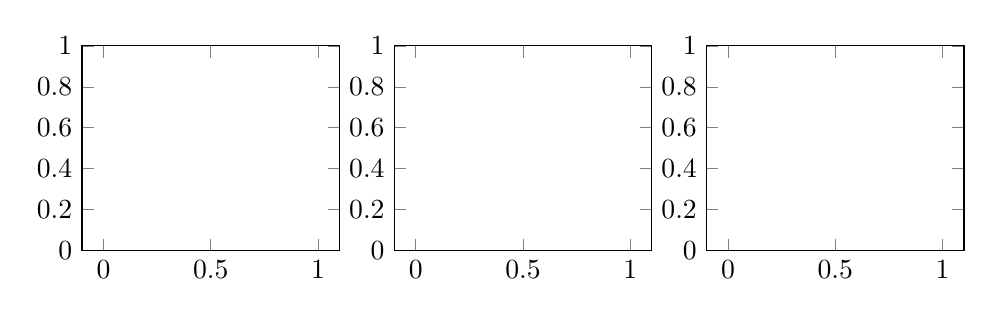
\begin{tikzpicture}

    \begin{axis}[%
            name=plot1,
            width=0.4\linewidth,
            ymin=-0.5, 
            ymax=0]
    \end{axis}

    \begin{axis}[%
            name=plot2,
            width=0.4\linewidth,
            at=(plot1.right of south east), anchor=left of south west,
            ymin=-6.5, ymax=0.2]
    \end{axis}

    \begin{axis}[%
            name=plot3,
            width=0.4\linewidth,
            at=(plot2.right of south east), anchor=left of south west,
            ymin=-6.5, ymax=0.2]
    \end{axis}

\end{tikzpicture}

\newpar{}
\ptitle{Angular Solutions} $\mathbf{Y}$

The two angular solutions combined are called \textbf{spherical harmonics}.
\begin{equation*}
    Y_{\ell}^{m_\ell}(\theta, \phi) = \epsilon\sqrt{\frac{2\ell+1}{4\pi}\frac{(\ell-|m_\ell|)!}{(\ell+|m_\ell|)!}}\:e^{im_\ell\phi}\:P_{\ell}^{m_\ell}(\cos(\theta))
\end{equation*}
where
\begin{equation*}
    \epsilon = \begin{cases}
        {(-1)}^{m_\ell} & m_\ell > 0    \\
        1               & m_\ell \leq 0
    \end{cases}
\end{equation*}

The spherical harmonics are normalized and orthogonal.

\newpar{}
\ptitle{Radial Equation} $\mathbf{R}$

Due to the spherical symmetry the radial equation becomes
\begin{equation*}
    \frac{-\hbar^2}{2m}\:\frac{d^2u}{dr^2}+\underbrace{\left[V(r)+\frac{-\hbar^2}{2m}\frac{\ell(\ell+1)}{r^2}\right]}_{V_{\text{eff}}}u = Eu
\end{equation*}
with
\begin{equation*}
    u(r) = rR(r)
\end{equation*}
Where $V(r)$ is the potential energy function which depends on the system. A solution of the radial equation of the hydrogen atom is given in Section~\ref{H-atom}.

\newpar{}
\ptitle{Remark on Spherical Coordinates}
\begin{align*}
    \theta & = \text{polar angle}     \\
    \phi   & = \text{azimuthal angle} \\
    r      & = \text{radius}
\end{align*}
\begin{align*}
    \mathbf{\nabla} & =\mathbf{u}_{r}\frac{\partial}{\partial r}+\frac{\mathbf{u}_{\theta}}{r}\frac{\partial}{\partial\theta}+\frac{\mathbf{u}_{\phi}}{r\sin\theta}\frac{\partial}{\partial\phi}                                      \\
    \nabla^2        & =\frac{1}{r^2}\frac{\partial}{\partial r}\left(r^2\frac{\partial}{\partial r}\right) + \frac{1}{r^2\sin(\theta)}\frac{\partial}{\partial\theta}\left(\sin(\theta)\frac{\partial}{\partial \theta}\right) \ldots \\
                    & + \frac{1}{r^2\sin^2(\theta)}\left(\frac{\partial^2}{\partial \phi^2}\right)
\end{align*}
\begin{equation*}
    d^3\mathbf{r} = dx\:dy\:dz = r^2\sin(\theta)dr\:d\theta\:d\phi
\end{equation*}

\textbf{Normalization}

\noindent\begin{equation*}
    \int_0^{2\pi}\int_0^{\pi} |Y_\ell^{m_\ell}|^2 \sin\theta\;d\theta d\phi \overset{!}{=} 1
\end{equation*}

\textbf{Orthogonality}

\noindent\begin{equation*}
    \int_0^{2\pi}\int_0^{\pi} {(Y_\ell^{m_\ell})}^{(a)}{(Y_\ell^{m_\ell})}^{(b)} \sin\theta\;d\theta d\phi \overset{!}{=} \begin{cases}
        1 & a=b     \\
        0 & a\neq b
    \end{cases}
\end{equation*}

\textbf{Remark}

Explicit solutions for the first few solutions of $Y_l^{m_l}$ can be found in the \textit{Useful Info Sheet}.

\subsection{Hydrogen Atom}\label{H-atom}
The potential energy function, i.e. $\widehat{V}(\mathbf{r})$, is \textbf{spherically symmetric} with respect to the nucleus. Therefor the SE in polar coordinates, stated in Section~\ref{3dSE_spherical_symmetry} can be used.
\newpar{}
The Coulombic attraction between the electron and the proton gives the potential energy function
\begin{equation*}
    V(r) = \frac{-e^2}{4\pi\epsilon_0}\frac{1}{r}
\end{equation*}

\ptitle{Radial Solution}

The solution to the radial part of the 3D SE becomes
\begin{align*}
    R_{n\ell}(r) = & \sqrt{{\left(\frac{2}{na}\right)}^3\frac{(n-\ell-1)!}{2n{[(n+\ell)!]}^3}} \ldots                    \\
                   & \ldots\exp\left(\frac{-r}{na}\right){\left(\frac{2r}{na}\right)}^\ell L_{n-\ell-1}^{2\ell+1}(2r/na)
\end{align*}
where $L_q^p (x)$ are the \textbf{associated Laguerre functions}, $n$ is the \textbf{principal quantum number} and $a$ is the Bohr radius.
\begin{equation*}
    a = \frac{4\pi\epsilon_0\hbar^2}{m_e e^2}=0.529 \cdot 10^{-10}m
\end{equation*}
where $m_e\simeq m$

\ptitle{Final Solution}

Combining the radial and the angular solution we get
\begin{equation*}
    \psi_{n\ell m_\ell}(r,\theta,\phi) = R_{n\ell}(r)\:Y_\ell^{m_\ell}(\theta, \phi)
\end{equation*}

where the quantum numbers are in the ranges of

\newpar{}
\textbf{principal quantum number} $n$
\noindent\begin{equation*}
    n = 1, 2, 3, \ldots
\end{equation*}
\begin{itemize}
    \item $n$ defines the energy level of an electron and thus the size of the electron cloud and the energy associated with the electrons orbit.
\end{itemize}

\newpar{}
\textbf{azimuthal quantum number} $\ell$
\noindent\begin{equation*}
    \ell = 0, 1, 2, \ldots , n-1
\end{equation*}
\begin{itemize}
    \item $\ell$ determines the shape of the electrons orbit ($\ell$ is the number of angular nodes).
    \item $\ell$ is directly related to the orbital angular momentum.
    \item $n-\ell-1$ is the number of radial nodes
\end{itemize}

\newpar{}
\textbf{magnetic quantum number} $m_\ell$
\noindent\begin{equation*}
    m_\ell =-\ell, -\ell+1, \ldots , \ell-1, \ell
\end{equation*}
\begin{itemize}
    \item $m_l$ describes the orientation of the angular momentum relative to an external magnetic field.
    \item $m_l$ is responsible for the magnetic splitting of spectral lines i.e.\ the \textit{Zeeman effect}
\end{itemize}

\begin{center}
    \includegraphics[width=\linewidth]{orbit_plots/hydrogen_orbit.jpg}
\end{center}

\newpar{}
\ptitle{Energies}

The Bohr formula gives the orbit energies of an H-atom.
\begin{equation*}
    E_n = -\left[\frac{m}{2\hbar^2}{\left(\frac{e^2}{4\pi\epsilon_0}\right)}^2\right]\frac{1}{n^2} = \frac{E_1}{n^2}
\end{equation*}
with $n \in \mathcal{N}$ and $E_1 = -13.6eV$

This is true for all \textit{hydrogenic} atoms. Note that the energy of the electronic level only depends on $n$.

\newpar{}
\ptitle{Degeneracy}

States are called \textit{degenerate} if they share their energy levels.
Considering the hydrogen atom with a given $n$ (except the ground state $n=1$), all states with $\ell=0,1,\ldots, n-1$ and $m_\ell=-\ell, \ldots, \ell$ are degenerate because they share their energy $E_n$.
\begin{center}
    \includegraphics[width=0.5\linewidth]{hydrogen_degeneracy.png}
\end{center}

\subsection{Cubical Infinite Square Well}
For the potential
\noindent\begin{equation*}
    V(x,y,z)=\begin{cases}0,&\text{if }x,y,z\text{ are all between }0\text{ and }a\\\infty,&\text{otherwise}\end{cases}
\end{equation*}
the stationary states $\Psi_n$ are given by

\noindent\begin{equation*}
    \Psi \left(x,y,z\right)={\left(\frac{2}{a}\right)}^{\frac{3}{2}} \sin\left(\frac{n_{x}\pi}{a}x\right)\sin\left(\frac{n_{y}\pi}{a}y\right)\sin\left(\frac{n_{z}\pi}{a}z\right)
\end{equation*}
and the corresponding energies are
\noindent\begin{equation*}
    E_n = \frac{\hbar^{2}}{2m} \frac{\pi^{2}}{a^{2}} \underbrace{\left(n_{x}^{2}+n_{y}^{2}+n_{z}^{2}\right)}_{n}
\end{equation*}

\section{Angular Momentum and Spin}
\subsection{Angular Momentum}

\ptitle{Operators}

From classical mechanics we derive
\begin{equation*}
    \hat{\mathbf{L}}=
    \begin{pmatrix}
        \hat{L_x} \\
        \hat{L_y} \\
        \hat{L_z}
    \end{pmatrix}
    =\hat{\mathbf{r}}\times\hat{\mathbf{p}}
    =
    \begin{pmatrix}
        y\widehat{p_z}-z\widehat{p_y} \\
        z\widehat{p_x}-x\widehat{p_z} \\
        x\widehat{p_y}-y\widehat{p_x}
    \end{pmatrix}
    =\frac{\hbar}{i}(\mathbf{\hat{r}}\times\hat{\mathbf{\nabla}})
\end{equation*}
with
\begin{equation*}
    |\mathbf{L}|=\sqrt{L_{x}^{2}+L_{y}^{2}+L_{z}^{2}}
\end{equation*}

\ptitle{Remarks}

\begin{itemize}
    \item $\widehat{L_x}, \widehat{L_y}, \widehat{L_z}$ are incompatible
    \item $\hat{L^2}$ and $\widehat{L_x}, \widehat{L_y}, \widehat{L_z}$ are compatible
    \item Various angular momentum commutators can be found in the appendix: ~\ref{comm_am}
\end{itemize}

\subsubsection{Ladder Operators for Angular Momentum}

Similar to the harmonic oscillator one can find the \textbf{ladder operators}
\begin{equation*}
    \widehat{L_{\pm}}=\widehat{L_{x}}\pm i \widehat{L_y}
\end{equation*}
which increase or lower the eigenvalue of $\widehat{L_{z}}$ by $\hbar$. These operators can be used to find the eigenvalues of angular momentum.

\subsubsection{Eigenfunctions}

As they are compatible (share eigenfunctions), we choose to find the eigenfunctions for $\widehat{L^2}$ and $\widehat{L_z}$
\begin{align*}
    \widehat{L^2}f_{\ell}^{m_l} & =\hbar^{2}\ell (\ell+1) f_{\ell}^{m_l} \\
    \widehat{L_z}f_{\ell}^{m_l} & =\hbar mf_{\ell}^{m_l}
\end{align*}
with quantum numbers
\begin{align*}
    \ell & =0, 1/2, 1, 3/2,\ldots                \\
    m    & =-\ell, -\ell+1, \ldots, \ell-1, \ell
\end{align*}
and the orthogonal \textbf{eigenfunctions}
\begin{equation*}
    f_{\ell}^{m_l}=Y_{\ell}^{m_l}
\end{equation*}
i.e. the spherical harmonics.

\ptitle{Remarks}

\begin{itemize}
    \item For each $l$ we have $2l+1$ values for $m_l$
    \item The eigenvalues are found by using the ladder method
    \item $Y_{\ell}^{m_l}$ are eigenfunctions of hermitian operators ($\widehat{L^2}$, $\widehat{L}_{z}$) and have \textbf{different eigenvalues}. Therefore, they are \textbf{orthogonal}.
\end{itemize}

\ptitle{Derivation}

Using $\nabla$ in spherical coordinates we get
\begin{equation*}
    \hat{\mathbf{L}}=\frac{\hbar}{i}\Bigg(\mathbf{u}_{\phi}\frac{\partial}{\partial\theta}-\mathbf{u}_{\theta}\frac{1}{\sin\theta}\frac{\partial}{\partial\phi}\Bigg)
\end{equation*}
and
\begin{align*}
    \widehat{L_{x}} & =-i\hbar\left(-\sin\phi\frac{\partial}{\partial\theta}-\cos\phi\cot\theta\frac{\partial}{\partial\phi}\right)                                                                        \\
    \widehat{L_{y}} & =-i\hbar\left(+\cos\phi\frac{\partial}{\partial\theta}-\sin\phi\cot\theta\frac{\partial}{\partial\phi}\right)                                                                        \\
    \widehat{L_{z}} & =\frac{\hbar}{i}\frac{\partial}{\partial\phi}                                                                                                                                        \\
    \hat{L}^{2}     & =-\hbar^{2}\left[\frac{1}{\sin\theta}\frac{\partial}{\partial\theta}(\sin\theta\frac{\partial}{\partial\theta})+\frac{1}{\sin^{2}\theta}\frac{\partial^{2}}{\partial\phi^{2}}\right]
\end{align*}
where combining the $\widehat{L_{i}}$ yields $\hat{L}^{2}$. Applying $\widehat{L_{z}}$ and $\hat{L}^{2}$ to the eigenvalue equations we find that the equations become equivalent to the \textbf{angular equation} from the hydrogen atom and hence, have the same eigenfunctions.

\subsubsection{Physical Interpretation}
As derived for the hydrogen atom, a single electron orbiting around a nucleus is described by $\psi_{n\ell m_\ell}(r,\theta,\phi)$ (having three quantum numbers $n,l,m_l$). The electron's angular momentum is described by the quantum numbers $l,m_l$. Given the eigenvalues of $\hat{L^2}$ and $\hat{L_z}$ we find the expectations
\begin{align*}
    |\mathbf{L}| & =\hbar\sqrt{l(l+1)} \\
    L_{z}        & =m_{l}\hbar
\end{align*}
as $m=-l,-l+1,\dots,l-1,l$ we conclude that $L_{z}$
\begin{itemize}
    \item Can only take discrete values
    \item Is always shorter than $|\mathbf{L}|$
    \item Can never point directly along the $z$ axis
\end{itemize}
As $L_x, L_y, L_z$ are incompatible we conclude that
\begin{itemize}
    \item We can determine $|\mathbf{L}|$ and $L_{z}$ simultaneously.
    \item But then have uncertainty in $L_x, L_y$.
\end{itemize}
Given a certain $l$, angular momentum can be described by a cone for each $m_l$
\begin{center}
    \includegraphics[width = 0.6\linewidth]{angular_momentum.png}
\end{center}

\subsection{Spin}
Similar to the earth having an angular momentum w.r.t. the sun but also itself, an electron has an angular momentum w.r.t. the nucleus and itself.

\ptitle{Operators}

$\hat{\mathbf{S}}$ follows the same rules as $\hat{\mathbf{L}}$ (see appendix ~\ref{comm_am_sp})

\ptitle{Remarks}

\begin{itemize}
    \item Electrons have an intrinsic spin.
    \item An electron \textbf{acts as if} it was rotating on an axis but it is not as it is zero-dimensional.
    \item This can easily be imagined as a spinning ball that is not a ball and does not spin.
\end{itemize}


\subsubsection{Eigenvalue Equation for Spin}
For a QM particle (not necessarily an electron) with spin one has
\begin{align*}
    \widehat{S^2}f_{s}^{m_s}   & =\hbar^{2}s (s+1) f_{s}^{m_s} \\
    \widehat{S_{z}}f_{s}^{m_s} & =\hbar m_sf_{s}^{m_s}
\end{align*}
where
\begin{align*}
    s   & =0,\frac{1}{2},1,\frac{3}{2},\dots \\
    m_s & =-s, -s+1,\dots, s-1, s
\end{align*}
i.e. angular momenta are restricted to integer and half-integer values.

\ptitle{Set Value for $\mathbf{s}$}

In contrast to angular momentum of a QM particle where $l$ could take arbitrary integer values, $s$ takes \textbf{a set value} for each particle.

\ptitle{Remarks}

\begin{itemize}
    \item For electrons we have $s=\frac{1}{2}$, for photons $s=1$
    \item Electrons have
          \begin{itemize}
              \item $m_s=\frac{1}{2}$ (spin up)
              \item $m_s=-\frac{1}{2}$ (spin down)
              \item Therefore, only two eigenstates $f_{\frac{1}{2}}^{\pm \frac{1}{2}}$
          \end{itemize}
\end{itemize}

\subsubsection{The State of Spin of an Electron}
As eigenstates for spin are not functions of $r,\theta, \phi$ (particle is zero-dimensional) one cannot write them as mathematical formulae for $f_{s}^{m_s}$. Instead, one uses Dirac notation:
\begin{equation*}
    f_{s}^{m_{s}}\rightarrow|s,m_{s}\rangle
\end{equation*}

\ptitle{Spin of an Electron}

For an electron with $s=\frac{1}{2}$, the eigenfunctions can be described by ket and bra as:
\begin{align*}
    f_{\frac{1}{2}}^{+\frac{1}{2}} & \rightarrow\left|\frac{1}{2},\quad +\frac{1}{2}\right>= \left|\uparrow\right>   \\
    f_{\frac{1}{2}}^{-\frac{1}{2}} & \rightarrow\left|\frac{1}{2},\quad-\frac{1}{2}\right> = \left|\downarrow\right>
\end{align*}
and one has
\begin{align*}
    |\mathbf{S}| & =\sqrt{\frac{1}{2}\left(\frac{1}{2}+1\right)}\hbar=\sqrt{\frac{3}{4}}\hbar \\
    S_z          & =\pm \frac{1}{2}\hbar
\end{align*}

\ptitle{General Spin State}

Spin can be in a general state

\begin{equation*}
    \left|\lambda\right>=a\left|\frac{1}{2},\quad +\frac{1}{2}\right>+b\left|\frac{1}{2},\quad -\frac{1}{2}\right>
\end{equation*}
where the probability of measuring a certain spin (assuming $\left|\lambda\right>$ \textbf{normalized}!) is given by $|a|^2$ for $\uparrow$ and $|b|^2$ for $\downarrow$ respectively.

\ptitle{Spin Operators as Matrices}

Setting the two eigenstates of the electron as basis vectors of a \textbf{two-dimensional} vector space we get

\begin{align*}
    \left|\frac{1}{2},\quad +\frac{1}{2}\right> & \rightarrow \left(\begin{matrix}
                                                                            1 \\
                                                                            0
                                                                        \end{matrix}\right) \\
    \left|\frac{1}{2},\quad -\frac{1}{2}\right> & \rightarrow \left(\begin{matrix}
                                                                            0 \\
                                                                            1
                                                                        \end{matrix}\right)
\end{align*}
Defining spin up and spin down \textbf{relative to z-axis} we get (by solving eigenvalue equation in Dirac notation):
\begin{align*}
    \hat{S}^2   & \rightarrow \frac{3}{4}{\hbar}^2\begin{bmatrix}
                                                      1 & 0 \\
                                                      0 & 1
                                                  \end{bmatrix} \\
    \hat{S}_{x} & \rightarrow \frac{\hbar}{2}\begin{bmatrix}
                                                 0 & 1 \\
                                                 1 & 0
                                             \end{bmatrix}      \\
    \hat{S}_{y} & \rightarrow \frac{\hbar}{2}\begin{bmatrix}
                                                 0 & -i \\
                                                 i & 0
                                             \end{bmatrix}      \\
    \hat{S}_{z} & \rightarrow \frac{\hbar}{2}\begin{bmatrix}
                                                 1 & 0  \\
                                                 0 & -1
                                             \end{bmatrix}      \\
\end{align*}

Note that
\begin{itemize}
    \item $\hat{S}_{x}$, $\hat{S}_{y}$ are non-diagonal i.e. the basis vectors are not eigenvectors of these operators.
    \item If they were diagonal in z-basis, $\hat{S}_{x},\hat{S}_{y},\hat{S}_{z}$ would have the same eigenvectors (but is not the case as they are incompatible).
\end{itemize}

\ptitle{Ladder Operators for Spin}

The ladder operators have the effect
\begin{align*}
    \hat{S}_{+}\left|\frac{1}{2},-\frac{1}{2}\right> & =\hbar\left|\frac{1}{2},+\frac{1}{2}\right> & \text{ (raises $S_z$ by $\hbar$)} \\
    \hat{S}_{-}\left|\frac{1}{2},+\frac{1}{2}\right> & =\hbar\left|\frac{1}{2},-\frac{1}{2}\right> & \text{ (lowers $S_z$ by $\hbar$)}
\end{align*}
and are in z-axis basis given by the \textbf{non-hermitian} matrices
\begin{align*}
    \hat{S}_{+} & \rightarrow \hbar\begin{bmatrix}
                                       0 & 1 \\
                                       0 & 0
                                   \end{bmatrix} \\
    \hat{S}_{-} & \rightarrow \hbar\begin{bmatrix}
                                       0 & 0 \\
                                       1 & 0
                                   \end{bmatrix}
\end{align*}


    \section{Formalism}

\subsection{Dirac Notation and Hilbert Spaces}
Assuming the functions $\alpha, \beta$ are square integrable i.e.\ in $L_2$ (\textbf{Hilbert space}) $\mathcal{H}$,
Dirac notation is used to simplify the notation of vectors, inner product (scalar product), expectation values etc. For the functions
\begin{align*}
    f   & = \sum_n c_n f_n     \\
    f^* & = \sum_n c_n^* f_n^*
\end{align*}
we define:
\noindent\begin{align*}
    |f\rangle           & := \begin{bmatrix}
                                 c_1 & c_2 & \cdots & c_n
                             \end{bmatrix}^T                               &  & \text{``ket''}              \\
    \langle f|          & := \begin{bmatrix}
                                 {c_1}^* & {c_2}^* & \cdots & {c_n}^*
                             \end{bmatrix}                   &  & \text{``bra''}                            \\
    \langle f|g \rangle & := \int_{-\infty}^{\infty} f^* g\; d \mathbf{r} \in L_2 &  & \text{inner product}
\end{align*}
where ``ket'' and ``bra'' are \textbf{vectors} that represent the function $f$.

These functions can be used as a complete orthonormal base (ONB) if
\noindent\begin{align*}
    \langle f_m|f_n \rangle & = \delta_{mn}                    &  & \text{orthonormal}        \\
    f(x)                    & = \sum_{n=1}^{\infty} c_n f_n(x) &  & \text{complete}           \\
    c_n                     & = \langle f_n|f \rangle          &  & \text{projection on base}
\end{align*}

\textbf{Remark}

Properites of the inner product can be found in Appendix\ \ref{ssec:InnerProd}

\subsubsection{Properties of QM Hilbert Space}
\begin{itemize}
    \item Describes \textbf{physical} solutions to QM systems
    \item The stationary states $\psi_n$ form an ONB and are complete
\end{itemize}

\subsection{Observables}
Observables are represented by hermitian operators.
\subsubsection{Hermitian Operators}
The expectation value of a observable is real and thus
\noindent\begin{align*}
    \langle Q\rangle           & = {\langle Q\rangle}^*                       \\
    \langle f|\hat{Q} g\rangle & = \langle \hat{Q}f|g\rangle\quad \forall f,g
\end{align*}
Such an operator is called a hermitian operator (applying the operator to one or the other member of an inner product yields the same result). An operator \textbf{must} be hermitian for its observable to become real. These operators are \textbf{linear} if
\noindent\begin{equation*}
    \hat{Q}\left[af(x)+bg(x)\right]=a\hat{Q}f(x)+b\hat{Q}g(x),
\end{equation*}

\ptitle{Properties}

\noindent\begin{align*}
    \langle f|(\hat{Q} + \hat{R})g\rangle                                    & = \langle (\hat{Q} + \hat{R})f|g\rangle                                                               \\[0.75em]
    \langle f|\hat{Q}\hat{R}g\rangle       =\langle \hat{Q}f|\hat{R}g\rangle & =  \langle \hat{R}\hat{Q}f|g\rangle \overset{[\hat{Q},\hat{R}]=0}{=} \langle \hat{Q}\hat{R}f|g\rangle
\end{align*}

\subsubsection{Determinant States}
A state $\Psi$ that would return the same result for every measurement of an ensemble is called a \textbf{determinant state} of the observable $Q$.
In other words, there would be no variance
\noindent\begin{align*}
    \sigma^2     & = \langle \Psi|(\hat{Q} - q) \Psi\rangle = 0 \\
    \hat{Q} \Psi & = q \Psi
\end{align*}
These determinant states of $Q$ are \textit{eigenfunctions} of $\hat{Q}$ and the expectation $\langle Q\rangle = q$ the corresponding \textit{eigenvalue}.
\newpar{}
In short: If a state fulfils the eigenvalue equation, every measurement will yield $q$.

\textbf{Remarks:}
\begin{itemize}
    \item A set of eigenvalues $q$ for $\hat{Q}$ is called its \textit{spectrum}.
    \item If multiple eigenfunctions share their eigenvalue, they are called \textit{degenerated states}.
    \item Eigenfunctions (of a Hermitian operator) with different eigenvalues are orthogonal and form a complete set.
    \item The TISE is an example for a determinant state\newline
          $\hat{Q}: \hat{H},\; q:E$.
\end{itemize}

\subsection{Eigenfunctions of a Hermitian Operator}
Eigenfunctions of hermitian operators can either have a discrete or continuous spectrum. For a discrete spectrum there are countably many eigenfunction whereas for a continuous the set of eigenfunctions is discrete as well.

\newpar{}
\ptitle{Discrete Spectrum}

If $\psi_n$ are solutions to $\hat{Q}\psi_n=q\psi_n$ then
\noindent\begin{align*}
    \Psi(x,0)    & = \sum_{n=1}^{\infty} c_n \underbrace{\psi_n(x)}_{\textsf{eigenfunctions}}    \\
    |\Psi\rangle & = \sum_{n=1}^{\infty} c_n \underbrace{|\psi_n\rangle}_{\textsf{eigenvectors}}
\end{align*}

\begin{itemize}
    \item Eigenvalues are real
    \item The eigenfunctions form a countable set (e. g. harmonic oscillator)
    \item Eigenfunctions with different eigenvalues are orthogonal
    \item Eigenfunctions with a discrete spectrum are within the Hilbert space $\mathcal{H}$, represent \textbf{physical} states and form a complete set.
    \item $|\psi_n\rangle$ can be thought of as basis vectors
\end{itemize}

\ptitle{continuous Spectrum}

\begin{itemize}
    \item Eigenfunctions with a continuous spectrum are not normalizable
    \item The eigenfunctions appear as continuous set (e.g. free particle)
    \item These eigenfuntions with real eigenvalues are \textit{Dirac-orthonormalizable} and form a \textbf{complete set}.
    \item In contrast to the discrete spectrum case where we had $\langle f_m|f_n\rangle=\delta_{mn}$ we now have
          \noindent\begin{equation*}
              \langle f_{x'}|f_{x''}\rangle=\delta(x''-x')
          \end{equation*}
\end{itemize}

\subsection{Generalized Statistical Interpretation}
If the spectrum of $\hat{Q}$ is discrete and the state
\begin{equation*}
    \Psi=\sum_n c_n f_n
\end{equation*}
is \textbf{not a eigenfunction} of $\hat{Q}$ (but $f_n$ is), the probability of measuring the particular eigenvalue $q_n$ corresponding to the eigenfunction $f_n(x)$ is
\noindent\begin{equation*}
    |c_n|^2, \quad c_n = \langle f_n|\Psi\rangle
\end{equation*}
It follows that
\noindent\begin{align*}
    \langle Q\rangle & = \langle\Psi_{general}|\hat{Q}\Psi_{general}\rangle                                                                 \\
                     & =\left(\sum_{m}c_{m}^{*}\langle\Psi_{m}|\right)\hat{Q}\left(\sum_{n}c_{n}|\Psi_{n}\rangle\right)                     \\
                     & = \sum_{n=1}^{\infty} |c_n|^2 q_n                                                                                    \\
    1                & =\sum_{n=1}^{\infty} |c_n|^2                                                                     & \text{normalized} \\
    \sigma^2         & \neq 0
\end{align*}
As mentioned in Section\ \ref{ssec:ISW}, these coefficients can be obtained by projecting $\Psi$ onto $\psi_n$:
\noindent\begin{equation*}
    c_n = \int_{-\infty}^{\infty} {\psi_n}^* \Psi\; d^3 \mathbf{r} = \langle \psi_n |\Psi \rangle
\end{equation*}

\textbf{Important Remark}

After a measurement of an observable, the wave function \textbf{collapses} into the measured eigenfunction $\psi_n$ with eigenvalue $q_n$ and probability $|c_n|^2$. This collapse reflects the transition from a superposition of possible states to a \textbf{definitive state}.

\subsection{Postulates of Quantum Mechanics}

\begin{enumerate}
    \item The state of a QM system is described by $\Psi(\mathbf{r},t)$, and $|\Psi|^2\; d^3 \mathbf{r}$ is the probability of finding the particle in the volume $d^3 \mathbf{r} = dx\,dy\,dz$.
    \item Every observable quantity in classical mechanics is represented by a \textbf{linear hermitian operator}, $\hat{Q}$, such that the mean value of the observable from an ensemble is
          \noindent\begin{equation*}
              \langle Q\rangle=\int\Psi^{*}\hat{Q}\Psi d^{3} \mathbf{r}= \langle\Psi|\hat{Q}\Psi\rangle
          \end{equation*}\newline
          \textbf{Restated}:\newline
          If the system is in a state that is an eigenstate of $\hat{Q}$, a measurement on a QM ensemble will always yield the eigenvalue $q$ of $\hat{Q}$ (e.g. determinant state of the infinite square well).\newline
          Else, a single measurement will yield one of the eigenvalues $q_n$ of $\hat{Q}$ with probability $|c_n|^2$ (e.g. general state of infinite square well).
    \item $\Psi(\mathbf{r},t)$ evolves in time according to the TDSE:
          \noindent\begin{align*}
              i\hbar \frac{\partial \Psi}{\partial t} & =\hat{H}\Psi                     \\
              \hat{H}                                 & = \frac{\hat{p}^2}{2m} + \hat{V}
          \end{align*}
\end{enumerate}

\subsection{Operators with Continuous Sets of Eigenfunctions}
Remember: these eigenfunctions are not normalizable (not in Hilbert space) but those of them with real eigenvalues are Dirac-orthonormalizable and form a complete set.

\subsubsection{Continuous Set of Eigenfunctions for Position}

\ptitle{Eigenvalue Equation}

An eigenfunction of the position operator must fulfil the following eigenvalue equation for a specific $x'$:
\begin{equation*}
    \hat{x}g_{x'} =x'g_{x'}
\end{equation*}
and hence,
\begin{equation*}
    x \cdot g_{x'} =x' \cdot g_{x'}
\end{equation*}

\ptitle{Eigenfunctions}

The eigenfunction
\begin{equation*}
    g_{x'}=\delta(x-x')
\end{equation*}
satisfies the stated eigenvalue equation as
\begin{equation*}
    x\cdot \delta(x-x')=x'\cdot \delta(x-x')
\end{equation*}
which means that measuring the position of a particle in state $g_{x'}$ (not physical) would always yield position $x'$.

\ptitle{Dirac-Orthonormality}

One can easily show that
\begin{equation*}
    \langle g_{x'}|g_{x''}\rangle=\delta(x''-x')
\end{equation*}

\ptitle{Completeness}

Any function $f$ can be written (as an infinite linear combination of eigenfunctions) in terms of $g_{x'}$:
\begin{equation*}
    \int_{-\infty}^{\infty}f(x^{\prime})g_{x^{\prime}}(x)dx^{\prime}=\int_{-\infty}^{\infty}f(x^{\prime})\delta(x-x^{\prime})dx^{\prime}=f(x)
\end{equation*}
where the coefficients are just given by the values of $f$ at the desired location i.e. $f(x')$.

\ptitle{Remarks}

\begin{itemize}
    \item In the discrete case the integral was a sum, $f(x')$ was $c_n$
\end{itemize}

\subsubsection{Continuous Set of Eigenfunctions for Momentum}

\ptitle{Eigenvalue Equation}

An eigenfunction of the momentum operator must fulfil the following eigenvalue equation for a specific $p'$:
\begin{equation*}
    \hat{p}f_{p^{\prime}}=p^{\prime}f_{p^{\prime}}
\end{equation*}

\ptitle{Eigenfunctions}

Plugging $\hat{p}=-i\hbar \frac{d}{dx}$ into the eigenvalue equation and solving the ODE yields waves with $k=\frac{2 \pi}{\lambda}=\frac{p'}{\hbar}$ and wavelength $\lambda=\frac{2\pi\hbar}{p^{\prime}}=\frac{h}{p^{\prime}}$ (de Broglie formula!):
\begin{equation*}
    f_{p^{\prime}}(x)=\frac{1}{\sqrt{2\pi\hbar}}\exp\left[\frac{ip^{\prime}x}{\hbar}\right]
\end{equation*}
which means that measuring the momentum of a particle in state $f_{p^{\prime}}(x)$ will always yield momentum $p'$.

\ptitle{Dirac-Orthonormality and Completeness}

As for $\hat{x}$ one can also show for $\hat{p}$ that
\begin{itemize}
    \item $\langle f_{p'}|f_{p''}\rangle=\delta(p''-p')$
    \item and $f_{p'}$ form a complete set
\end{itemize}


\subsection{The Generalized Uncertainty Principle}
\subsubsection{Compatible and Incompatible Observables}

\ptitle{Compatible Observables}

\begin{itemize}
    \item The operators do commute
    \item The operators have the same eigenfunctions
    \item Hence, the two observables can be determined simultaneously i.e. for some general state $\psi$, measuring a $A$ yields a certain eigenvalue $a_n$ with probability $|c_{n,A}|^2$ and subsequent measurement of $A$ will yield $a_n$ too. The wave function is now collapsed into a certain eigenfunction $\psi'$ of $A$ which, as we said, is an eigenfunction of $\hat{B}$ too (with eigenvalue $b_m$). Therefore: measuring $A$ is now deterministic (yields $a_n$) \textbf{and} subsequent measurement of $B$ is deterministic too (yields $b_m$): The two observables can simultaneously be determined arbitratrarily precisely without any uncertainty in either one of them.
\end{itemize}

\ptitle{Incompatible Observables}

\begin{itemize}
    \item The operators don't commute
    \item The operators don't have the same eigenfunctions
    \item The two observables can't be determined simultaneously i.e. for some general state $\psi$, measuring a $A$ yields a certain eigenvalue $a_n$ with probability $|c_{n,A}|^2$ and subsequent measurement of $A$ will yield $a_n$ too as the wave is collapsed into an eigenfunction of $\hat{A}$. However, as this is not an eigenfunction of $\hat{B}$, subsequent measurement of $B$ remains \textbf{probabilistic} (yields $b_m$ with probability $|c_{m,B}|^2$) which means that $A$ and $B$ can't simultaneously be determined without any uncertainty.
\end{itemize}

\subsubsection{General Uncertainty Principle (GUP) for Incompatible Operators}
For any Observables $A$, $B$:
\begin{equation*}
    \sigma_A^2\cdot\sigma_B^2\geqslant{\left(\frac1{2i}\langle[\hat{A},\hat{B}]\rangle\right)}^2
\end{equation*}

\ptitle{Remarks}

\begin{itemize}
    \item The quantity $\left(\frac1{2i}\langle[\hat{A},\hat{B}]\rangle\right)$ is real (and it's square hence positive).
    \item $\langle[\hat{A},\hat{B}]\rangle=\langle\Psi|\hat{A}\hat{B}\Psi\rangle-\langle\Psi|\hat{B}\hat{A}\Psi\rangle$
\end{itemize}

\begin{examplesection}[Example: Position and Momentum]
    For $\hat{A}=x$, $\hat{B}=-i\hbar d/dx$ we have
    \begin{align*}
        \left[\hat{x},\hat{p}\right] & =i\hbar                                                                      \\
        \sigma_{x}^{2}\sigma_{p}^{2} & \geq{\left(\frac{1}{2i}i\hbar\right)}^{2}={\left(\frac{\hbar}{2}\right)}^{2} \\                                                           \\
        \sigma_{x}\sigma_{p}         & \geq\frac{\hbar}{2}
    \end{align*}
\end{examplesection}

\subsubsection{Time-Energy Uncertainty}
Plugging the \textbf{generalized Ehrenfest theorem}
\begin{equation*}
    \frac{d}{dt}\left\langle Q\right\rangle=\frac{i}{\hbar}\left\langle\left[\hat{H},\hat{Q}\right]\right\rangle+\left\langle\frac{\partial\hat{Q}}{\partial t}\right\rangle
\end{equation*}
into the GUP yields, assuming $\hat{Q}$ is time-independent, the \textbf{time-energy uncertainty}:
\begin{equation*}
    \Delta t\cdot\Delta E\geqslant\frac\hbar2
\end{equation*}
where
\begin{align*}
    \Delta t & \equiv \frac{\sigma_Q}{|d\langle Q\rangle/dt|} \\
    \Delta E & \equiv \sigma H
\end{align*}

\ptitle{Remarks}

\begin{itemize}
    \item $\Delta t$ describes how long it takes the expectation value of $Q$ to change by $\sigma$.
    \item The generalized Ehrenfest theorem states that the rate of change of $\langle Q \rangle$ is determined by the commutator of the operator and the Hamiltonian.
    \item If they commute, $Q$ is a conserved quantity.
\end{itemize}
    \section{Multi-Particle Systems and Atoms}
\subsection{Two-Particle Systems}
\subsubsection{Properties Two-Particle Systems}
Again, we assume that $V$ is time-independent.

\newpar{}
\ptitle{Similarities to One-Particle Systems}

\begin{itemize}
    \item $\Psi$ describes system
    \item time dependence: TDSE
    \item total energy: TISE
    \item $\Psi_{gen}=\sum_{n} c_{n} \Psi_{n} \exp\left[\frac{-i E_{n} t}{\hbar}\right]$
\end{itemize}

\newpar{}
\ptitle{Differences to One-Particle Systems}
\begin{itemize}
    \item $\Psi(\mathbf{r_1},\mathbf{r_2},t)$ is a function of position of both particles
    \item $\widehat{H}$ is given by
          \begin{equation*}
              \widehat{H}=-\frac{\hbar^{2}}{2m_{1}}\nabla_{1}^{2}-\frac{\hbar^{2}}{2m_{2}}\nabla_{2}^{2}+V(\mathbf{r}_{1},\mathbf{r}_{2},t)
          \end{equation*}
          where $V$ includes any interactions between particles i.e.:
          \begin{enumerate}
              \item interactions between  electrons
              \item interactions of electrons with the nucleus
          \end{enumerate}
    \item The term
          \begin{equation*}
              |\Psi(\mathbf{r}_{1},\mathbf{r}_{2},t)|^{2} d^{3}\mathbf{r}_{1} d^{3}\mathbf{r}_{2}
          \end{equation*}
          describes the probability of finding particle 1 in volume $d^{3}\mathbf{r}_{1}$, particle 2 in volume $d^{3}\mathbf{r}_{2}$
\end{itemize}

\subsubsection{Z-Particle Systems}
In a general multi-particle system (e.g.\ atom with $Z$ protons) the Hamiltonian is given by
\begin{align*}
    \widehat{H} = & \underbrace{\sum_{j=1}^{Z}\left\{-\frac{\hbar^{2}}{2m}\nabla_{j}^{2}-\left(\frac{1}{4\pi \epsilon_{0}}\right)\frac{Ze^{2}}{r_{j}}\right\}}_{T\text{ and interaction with nucleus}} \\
    +             & \underbrace{\frac{1}{2}\left(\frac{1}{4\pi \epsilon_{0}}\right)\sum_{j\neq k}^{Z}\frac{e^{2}}{\left|\mathbf{r}_{j}-\mathbf{r}_{k}\right|}}_{\text{repulsive int.\ of electrons}}
\end{align*}
where in the ``repulsion'' term
\begin{itemize}
    \item the interaction between electrons $j,k$ is described
    \item $\frac{1}{2}$ avoids double counting due to permuting $j,k$
\end{itemize}
The ``repulsion'' term makes exact solving of the TISE, in general, impossible. An approximation and an exception are presented hereafter.

\subsubsection{Reduceable Two-Particle Problems}
In two special cases the TISE of two-particle systems can be solved analytically.

\newpar{}
\ptitle{1. Noninteracting Particles}

\begin{itemize}
    \item Corresponds to ignoring the ``repulsion'' term in $\widehat{H}$ of the Z-particle system
    \item Assume e.g.\ electrons only interact with nucleus but not each other (simplest but most inaccurate approximation)
    \item Each electron in single particle hydrogenic state: $\psi_{n,l,m_l,m_s}$
    \item See~\ref{ssec:NIP} for details
\end{itemize}

\newpar{}
\ptitle{2. Central Potential Systems}

Given a system where the particles interact only with each other via a potential that depends on their separation
\begin{equation*}
    V(\mathbf{r}_1,\mathbf{r}_2)\to V(|\mathbf{r}_1-\mathbf{r}_2|)
\end{equation*}
we can solve the two-particle TISE analytically by splitting the problem into center-of-mass motion
\begin{align*}
    \mathbf{R}\equiv\  & \frac{m_1\mathbf{r_1}+m_2\mathbf{r_2}}{m_1+m_2} &  & \text{ center of mass} \\
    M\equiv\           & m_1 + m_2                                       &  & \text{ total mass}
\end{align*}
and relative motion of the two particles
\begin{align*}
    \mathbf{r}\equiv\  & \mathbf{r_1}-\mathbf{r_2} &                      \\
    m_r\equiv\         & \frac{m_1 m_2}{m_1+m_2}   & \text{ reduced mass}
\end{align*}
In this case, the TISE separates to
\begin{equation*}
    -\frac{\hbar^{2}}{2M}\nabla_{\mathbf{R}}^{2}\psi-\frac{\hbar^{2}}{2m_r}\nabla_{\mathbf{r}}^{2}\psi+V(\mathbf{r})\psi=E\psi
\end{equation*}
and we can find a solution
\begin{equation*}
    \psi = \psi_\mathbf{R}(\mathbf{R})\cdot\psi_\mathbf{r}(\mathbf{r})
\end{equation*}
Remarks:
\begin{itemize}
    \item Works only for 2-particle system
    \item For the H-atom we calculated $\psi_\mathbf{r}(\mathbf{r})$ and assumed $m_r\approx m_e$ (plug it into $m_r$ to see why)
\end{itemize}

\subsubsection{Noninteracting Particles}\label{ssec:NIP}
As a coarse approximation we \textbf{ignore the ``repulsion'' term} from the n-particle TISE to neglect all electron-electron interactions. Then, for two given single-particle solutions $\psi_a$ and $\psi_b$ one differenciates between the following two cases.

\newpar{}
\ptitle{Distinguishable Particles}

The overall solutions are products
\begin{equation*}
    \psi(\mathbf{r}_{1},\mathbf{r}_{2})=\psi_{a}(\mathbf{r}_{1})\psi_{b}(\mathbf{r}_{2})
\end{equation*}
or
\begin{equation*}
    \psi(\mathbf{r}_{1},\mathbf{r}_{2})=\psi_{b}(\mathbf{r}_{1})\psi_{a}(\mathbf{r}_{2})
\end{equation*}
where
\begin{itemize}
    \item $\psi(\mathbf{r}_{1},\mathbf{r}_{2})$ is the overall, 2-particle wave function
    \item $\psi_{a}(\mathbf{r}_{1})$ means particle $1$ is in state $\psi_{a}$ etc.
\end{itemize}

\newpar{}
\ptitle{Indistinguishable Particles}

For the case of e.g.\ two electrons (which are indistinguishable) the overall 2-particle wave function is a \textbf{linear combination} of the aforementioned products:

\begin{equation*}
    \psi_{+}(\mathbf{r}_{1},\mathbf{r}_{2})=C\left[\psi_{a}(\mathbf{r}_{1})\psi_{b}(\mathbf{r}_{2})+\psi_{b}(\mathbf{r}_{1})\psi_{a}(\mathbf{r}_{2})\right]\quad \mathrm{symmetric}
\end{equation*}
or
\begin{equation*}
    \psi_{-}(\mathbf{r}_{1},\mathbf{r}_{2})=C\left[\psi_{a}(\mathbf{r}_{1})\psi_{b}(\mathbf{r}_{2})-\psi_{b}(\mathbf{r}_{1})\psi_{a}(\mathbf{r}_{2})\right]\quad \mathrm{antisymm.}
\end{equation*}
Remarks
\begin{itemize}
    \item Indistinguishable means that there is no way to  tell the two particles apart
    \item $\psi_{+}$ stays exactly the same when swapping $\mathbf{r_1},\mathbf{r_2}$
    \item $\psi_{-}$ changes sign when swapping $\mathbf{r_1},\mathbf{r_2}$
    \item Implications of these two solutions are presented subsequently
\end{itemize}

\paragraph[Exchange Symmetry of psi]{Exchange Symmetry of $\psi_{\pm}$}

\ptitle{Exchange Operator}

The exchange operator swaps two particles
\begin{equation*}
    \widehat{P}\psi(\mathbf{r_1},\mathbf{r_2})=\psi(\mathbf{r_2},\mathbf{r_1})
\end{equation*}
For two identical particles one has
\begin{align*}
    m_1=        & m_2        \\
    V(r_1,r_2)= & V(r_2,r_1)
\end{align*}
which means
\begin{equation*}
    \left[\widehat{P},\widehat{H}\right]=0
\end{equation*}
which by the generalized Ehrenfest theorem implies

\begin{equation*}
    \frac{d}{dt}\langle\widehat{P}\rangle=0
\end{equation*}
and means that $\widehat{P}$ and $\widehat{H}$ share the eigenfunctions $\psi_{\pm}$.

\ptitle{Exchange Symmetry of Noninteracting Particles}

One has that
\begin{itemize}
    \item $\psi_{+}$ is symmetric w.r.t.\ exchange (eigenvalue $+1$)
    \item $\psi_{-}$ is antisymmetric w.r.t.\ exchange (eigenvalue $-1$)
    \item $\psi_{\pm}$ are stationary states
    \item As $P$ is a conserved quantity a particle,\newline once (anti)symmetric w.r.t.\ exchange,\newline stays (anti)symmetric
\end{itemize}
For two \textbf{distinguishable} particles one finds that
\begin{equation*}
    \left\langle{\left(x_{1}-x_{2}\right)}^{2}\right\rangle_{d}=\left\langle x^{2}\right\rangle_{a}+\left\langle x^{2}\right\rangle_{b}-2\left\langle x\right\rangle_{a}\left\langle x\right\rangle_{b}
\end{equation*}
For two \textbf{undistinguishable} particles one has
\begin{align*}
    \left\langle{\left(x_{1}-x_{2}\right)}^{2}\right\rangle_{\pm}= & \left\langle x^{2}\right\rangle_{a}+\left\langle x^{2}\right\rangle_{b}-2\langle x\rangle_{a}\langle x\rangle_{b}\mp2|\langle x\rangle_{ab}|^{2} \\
                                                                   & =\left\langle{\left(\Delta x\right)}^{2}\right\rangle_{d}\mp2\left|\left\langle x\right\rangle_{ab}\right|^{2}
\end{align*}
Therefore, particles that are in state $\psi_{+}$ (symmetric w.r.t.\ exchange) tend to be closer together than particles that are in state $\psi_{-}$.\\
\textbf{Remarks}
\begin{itemize}
    \item $\left\langle\cdot\right\rangle_{d/\pm}$ is the expectationvalue in a distinguishable/indistinguishable state
    \item This phenomenon is often called ``exchange interaction'' or ``exchange force''
    \item Exchange symmetry or the overall 2-particle wave function influences location of particles w.r.t.\ each other
\end{itemize}

\paragraph{Bosons and Fermions}
\begin{itemize}
    \item \textbf{Bosons} (e.g.\ photons (s=1), gravitons (s=2)) are particles with \textbf{integer} spin
    \item \textbf{Fermions} (e.g.\ electrons, protons, neutrons (s=$\frac{1}{2}$)) are particles with \textbf{half-integer} spin
\end{itemize}
As bosons are indistinguishable (same holds for fermions) their overall wave functions behave according to the previously stated rules.

\ptitle{Exchange Symmetry Axiom}

The exchange symmetry of the overall wave function of
\begin{itemize}
    \item identical \textbf{bosons is symmetric} w.r.t.\ exchange
    \item identical \textbf{fermions is antisymmetric} w.r.t.\ exchange
\end{itemize}

\ptitle{Exchange Symmetry of Hydrogen}

Because electrons are fermions one
\begin{itemize}
    \item would intuitively choose $\psi_{-}$ as an overall wave function.
    \item must choose $\psi_{+}$ because $\psi_{-}$ would mean antibonding in $\mathrm{H}_2$.
\end{itemize}
One finds that spin also influences the overall wave function according to
\begin{equation*}
    \psi(\mathbf{r_1},\mathbf{r_2})=\psi(\mathbf{r})\chi(s)
\end{equation*}
and one has for $\chi(s)$ and two identical spins $s=\frac{1}{2}$ the spin states
\begin{align*}
     & \begin{rcases}
           \uparrow \uparrow                                                        \\
           \downarrow \downarrow                                                    \\
           \frac{1}{\sqrt{2}}\left(\uparrow \downarrow + \downarrow \uparrow\right) \\
       \end{rcases} \chi_{\mathrm{triplet}}(s)\text{: symmetric w.r.t.\ ex.} \\
     & \begin{rcases}
           \frac{1}{\sqrt{2}}\left(\uparrow \downarrow - \downarrow \uparrow\right)
       \end{rcases} \chi_{\mathrm{singlet}}(s) \text{: antisymmetric w.r.t.\ ex.}
\end{align*}
which implies that the overall wave function $\psi(\mathbf{r_1},\mathbf{r_2})=\psi(\mathbf{r})\chi(s)$ of hydrogen becomes
\begin{equation*}
    \psi_{+}\cdot \chi_{\mathrm{singlet}}(s)
\end{equation*}
to achieve a stable chemical bond.

\newpar{}
\textbf{Remarks}
\begin{itemize}
    \item $\psi_{-}\cdot \left(\text{triplet}\right)$ would also lead to antisymmetric $\psi(\mathbf{r_1},\mathbf{r_2})$ but is higher in energy because of antibonding.
\end{itemize}

\newpar{}
\ptitle{Pauli Exclusion Principle}

One cannot have two electrons in exactly the same state (same quantum numbers) and still have the system antisymmetric w.r.t.\ exchange because one then has $\psi_{-}=0$ i.e.\ there is no such state (Choose $\psi_{-}$ because electrons are fermions).

\subsection{Atoms}
\subsubsection{Hydrogen Orbitals}
\paragraph{Orbital Description by Quantum Numbers (QN)}
\renewcommand{\arraystretch}{1.1}
\setlength{\oldtabcolsep}{\tabcolsep}\setlength\tabcolsep{2pt}
{\small     % Smaller font
    \begin{tabularx}{\linewidth}{@{}lllX@{}}
              & \textbf{Name} & \textbf{Range|Letter}                             & \textbf{Meaning}    \\
        $n$   & principal QN  & $0|K,\;1|L,\;2|M,\dots$                           & shell (radius)      \\
        $l$   & azimuthal QN  & $0|s,\;1|p,\;2|d,\;3|f,\dots$                     & subshell            \\
              &               &                                                   & (orbital shape)     \\
        $m_l$ & magnetic QN   & $-l,-l+1,\dots,l-1,l$                             & orbital orientation \\
              &               &                                                   & \# of orientations  \\
        $m_s$ & spin QN       & $+\frac{1}{2}/\uparrow,\:-\frac{1}{2}/\downarrow$ & spin orientation    \\
              &               &                                                   & (w.r.t.\ z-axis)    \\
        $s$   & spin          & fermions: half-int                                &                     \\
              &               & bosons: int                                       &
    \end{tabularx}
}           % End smaller font
\renewcommand{\arraystretch}{1}
\setlength{\tabcolsep}{\oldtabcolsep}

\ptitle{Visualization}

\begin{center}
    \includegraphics[width = 0.75\linewidth]{shell_subshell_orbital.png}
\end{center}
\textit{source: chemistry stack exchange}
\begin{center}
    \includegraphics[width = 0.99\linewidth]{orbitals.png}
\end{center}

\ptitle{Remarks}

\begin{itemize}
    \item One sometimes also calls orbitals
          \begin{itemize}
              \item by their azimuthal QN, e.g.\ for $l=1$: ``p-orbitals''
              \item by their principal QN, e.g.\ for $n=2$: ``2p-orbitals''
          \end{itemize}
    \item Each orbital can contain \textbf{two electrons}, one with $m_s=+\frac{1}{2}$, one with $m_s=-\frac{1}{2}$ (Pauli: unique set of QN)
    \item An s-orbital with QN $n$ has $n-1$ radial nodes
\end{itemize}

\paragraph{Orbital Table}
\renewcommand{\arraystretch}{1.1}
\setlength{\oldtabcolsep}{\tabcolsep}\setlength\tabcolsep{3pt}
{\small     % Smaller font
    \begin{tabularx}{\linewidth}{@{}llllll@{}}
            &                &                      &                      & \multicolumn{2}{c}{\# \textbf{of electrons}\dots}                      \\
        $n$ & \textbf{Shell} & \textbf{Subshell(s)} & \# \textbf{Orbitals} & \textbf{per Subshell}                             & \textbf{per Shell} \\
        1   & K              & s                    & 1                    & 2                                                 & 2                  \\
        \cmidrule{1-6}
        2   & L              & s                    & 1                    & 2                                                 & 8                  \\
            &                & p                    & 3                    & 6                                                 &                    \\
        \cmidrule{1-6}
        3   & M              & s                    & 1                    & 2                                                 & 18                 \\
            &                & p                    & 3                    & 6                                                 &                    \\
            &                & d                    & 5                    & 10                                                &                    \\
        \cmidrule{1-6}
        4   & N              & s                    & 1                    & 2                                                 & 32                 \\
            &                & p                    & 3                    & 6                                                 &                    \\
            &                & d                    & 5                    & 10                                                &                    \\
            &                & f                    & 7                    & 14                                                &
    \end{tabularx}
}           % End smaller font
\renewcommand{\arraystretch}{1}
\setlength{\tabcolsep}{\oldtabcolsep}

\ptitle{Remarks}

\begin{itemize}
    \item The total number of orbitals is the number of possible states ($n,l,m_l$) that one electron can occupy.
    \item Including spin one can have two electrons per orbital.
\end{itemize}

\subsubsection{Filling Orbitals with Electrons}
The hydrogenic atom model is an atom with $Z$ protons and $1$ single electron.
\paragraph{Hydrogenic (One-Electron) Atoms}

\ptitle{Energy Levels}

\begin{center}
    \includegraphics[width = 0.75\linewidth]{hydr_energy_levels.png}
\end{center}
\begin{itemize}
    \item Reminder: $E_n = -\left[\frac{m}{2\hbar^2}{\left(\frac{e^2}{4\pi\epsilon_0}\right)}^2\right]\frac{1}{n^2} = \frac{E_1}{n^2}$
    \item States are degenerate: the energy only depends on $n$, so the 2s and 2p orbitals are on same level given $n$ for an 1-electron atom!
\end{itemize}

\paragraph{Multielectron (Non-Hydrogenic) Atoms}

\ptitle{Energy Levels}

\begin{center}
    \includegraphics[width = 0.6\linewidth]{multielectron_energy_levels.png}
\end{center}
\begin{itemize}
    \item Example of screening: 1s and 2s electrons neutralize a part of the influence of the nucleus on the p orbitals
          \begin{itemize}
              \item The energy states become non-degenerate due to electron-electron interactions
              \item s electrons are closer to nucleus: higher attraction to nucleus $\leftrightarrow$ lower in energy
              \item p electrons are further away due to screening: lower attraction to nucleus $\leftrightarrow$ higher in energy
          \end{itemize}
    \item Screening results in different energies depending on location of electron i.e.\ shape of subshell
\end{itemize}

\ptitle{Filling Energy Levels with Electrons}

As the shells overlap, one can not just assume that a larger $n$ yields a larger energy levels (e.g.\ $E_{4s}<E{3d}$). Therefore, one needs to follow a specific order when filling orbitals with electrons. One can either use the graphical method:
\begin{center}
    \includegraphics[width = 0.4\linewidth]{fill_energies_graphical.png}
\end{center}
\textit{source: http://hyperphysics.phy-astr.gsu.edu/}\\
or use the periodic table. Both yield the filling order
\begin{equation*}
    1s^2 2s^2 2p^6 3s^2 3p^6 4s^2 3d^{10}\dots
\end{equation*}

\ptitle{Noble Gas Notation}

Instead of writing all base orbitals down, even for atoms with large $Z$, one can initiate the electron configuration formula with the noble gas preceding the element in brackets.

\newpar{}
\textbf{Example}:
\begin{equation*}
    Fe(Z=26): 1s^2 2s^2 2p^6 3s^2 3p^6 4s^2 3d^6
\end{equation*}
can be rewritten as
\begin{equation*}
    Fe(Z=26): \left[Ar\right]4s^2 3d^6
\end{equation*}

\ptitle{Exceptions}

Some elements don't follow the general rules for filling orbitals. Two important examples are
\begin{equation*}
    Cr: \left[Ar\right]4s^1 3d^5
\end{equation*}
\begin{equation*}
    Cu: \left[Ar\right]4s^1 3d^{10}
\end{equation*}
which yields an energetically more optimal state.

\ptitle{Valence Electrons}

\begin{itemize}
    \item The chemical reactivity strongly depends on the \# of valence electrons (outermost shell)
    \item Noble (inert) gases have a full valence shell: don't react chemically
\end{itemize}

\subsubsection{Full-State Description of Atoms}

\begin{itemize}
    \item Full subshells give fixed contributions to the state of an atom.
    \item Non-full subshells have freedom in how to fill their orbitals with electrons. Therefore, one needs to establish a method to describe these states and answer the question ``in what orbital and spin angular momentum states are these electrons''?
    \item This method is especially useful when searching for the ground state of a certain atom.
\end{itemize}

\ptitle{Important Rules}

\begin{enumerate}
    \item \textbf{Filled subshells} never contribute to $L$, $S$, $J$.
    \item One can use the \textbf{addition rule} to find all possible combination of momentum cones.
    \item All the angular momentum quantum numbers ($l,s,\dots,L,S,\dots$) must be \textbf{multiplied by} $\boldsymbol{\hbar}$ to find the actual angular momenta.
\end{enumerate}

\paragraph{Total Momentum Quantum Numbers}

\ptitle{Angular Momentum (AM) in Multiparticle Systems}

One can establish a full-state description of an atom using total (orbital and spin) angular momentum. As these observables commute with $\hat{H}$ they are conserved quantities and useful for state description. For orbital angular momentum one defines
\begin{align*}
    L                   & \text{: total orbital AM}                \\
    M_L=\sum_{i}m_{l,i} & \text{: total orb. AM projection on $z$} \\
\end{align*}
For spin one has
\begin{align*}
    S                   & \text{: total spin AM}                    \\
    M_S=\sum_{i}m_{s,i} & \text{: total spin. AM projection on $z$} \\
\end{align*}
and in total one has
\begin{align*}
    J           & \text{: total AM}                   \\
    M_J=M_L+M_S & \text{: total AM projection on $z$} \\
\end{align*}

Remarks
\begin{itemize}
    \item For $M_L=0$ one also has $L=0$
    \item For $M_S=0$ one also has $S=0$
    \item $M_L$ relates to $L$ as $m_l$ relates to $l$ (i.e.\ $M_L$ is a projection of total angular momentum along $z$)
    \item $M_S$ relates to $S$ as $m_s$ relates to $s$
    \item One finds the possible values for $L,S,J$ using the addition rule.
\end{itemize}

\ptitle{Addition Rule}

Given two orbital or spin angular momenta $j_1, j_2$ one has
\begin{equation*}
    J=(j_1+j_2),\dots,|j_1-j_2|
\end{equation*}
with integer steps in between.\\
Remarks:
\begin{itemize}
    \item Describes combinations to fill partially-filled subshells (many possible combinations).
    \item Arises because AM are directional and quantized.
    \item Depending on the specific values for the $j_i$ one has half-integer, integer or multi-integer steps between possible $J$ (Caution: often not all in-between steps are taken)!
    \item Given ranges for $L$ and $S$ for an atom, one can choose a specific pair $(L,S)$ and apply the addition rule to get $J$ i.e.
          \begin{equation*}
              J=(L+S),\dots,|L-S|
          \end{equation*}
    \item Remember that for electrons one always has $s=+\frac{1}{2}$ but $m_s=\pm \frac{1}{2}$
\end{itemize}

\ptitle{Term Symbol}

As partially-filled subshells impose a range of possible atom states (ways to fill electrons in subshells) given by the combinations of the $L,S,J$ one defines a simplified notation given by
\begin{equation*}
    \prescript{2S+1}{}{X_J}
\end{equation*}
where one uses for $X$ the same letters as for the subshells
\begin{equation*}
    X=
    \begin{cases}
        S,     & L=0 \\
        P,     & L=1 \\
        D,     & L=2 \\
        \vdots &
    \end{cases}
\end{equation*}

Remarks
\begin{itemize}
    \item The superscript $2S+1$ stands for the \# of projections
    \item The special case of $2S+1=1$ is called singlet
    \item The special case of $2S+1=3$ is called triplet
\end{itemize}

\ptitle{Excange Symmetry}

\begin{itemize}
    \item The addition rule does not consider exchange symmetry (Pauli exclusion).
    \item Therefore, not all states $\prescript{2S+1}{}{X_J}$ found for a certain atom are antisymmetric w.r.t.\ exchange but one needs the latter for electrons!
    \item Some states would require 2 electrons with exactly the same quantum numbers.
    \item There are specific rules to find these valid states (not part of this course).
\end{itemize}

\ptitle{Hund's Rules for Finding Ground States}

After considering exchange symmetry, one has reduced the number of possible states. One can the apply Hund's rule to find the lowest-energy state called ``ground state''
\begin{enumerate}
    \item State with largest $S$ is most stable
    \item For states with same $S$, largest $L$ is most stable
    \item For states with same $S$ and $L$ (but different $J$)
          \begin{itemize}
              \item Smallest $J$ most stable for subshells that are no more than half full
              \item Larqest $J$ most stable for subshells that are more than half full
          \end{itemize}
\end{enumerate}


\section{Solids}
\subsection{Free-Electron Model}
Neglecting spin and electron-electron interactions, an electrons wavefunction in a box with length $l_x,l_y,l_z$ is given by
\noindent\begin{align*}
    E_{n_x,n_y,n_z}    & = \frac{\hbar^2\pi^2}{2m}\left(\frac{n_x^2}{l_x^2}+\frac{n_y^2}{l_y^2}+\frac{n_z^2}{l_z^2}\right),\quad n_x,n_y,n_z \in \mathbb{N}\backslash 0 \\
    \psi_{n_x,n_y,n_z} & = \sqrt{\frac{8}{l_x l_y l_z}} \sin\left(\frac{n_x\pi}{l_x}x\right) \sin\left(\frac{n_y\pi}{l_y}y\right) \sin\left(\frac{n_z\pi}{l_z}z\right)
\end{align*}
based on this solution of the SE, the distance between the discrete energy levels is at most
\noindent\begin{equation*}
    \Delta E \leq 10^{-6} ~\mathrm{eV}
\end{equation*}
and therefore the states from continous \textit{electron bands}.


\subsubsection{k-Space}
By transforming the energy into the k-space (wavenumbers), the energy becomes
\noindent\begin{equation*}
    E = \frac{\hbar^2k^2}{2m}, \quad \begin{cases}
        k^2 = k_x^2+k_y^2+k_z^2 \\
        k_x = \frac{n_x\pi}{l_x}, k_y = \frac{n_y\pi}{l_y}, k_z = \frac{n_z\pi}{l_z}
    \end{cases}
\end{equation*}
and each solution occupies
\noindent\begin{equation*}
    \frac{\pi^3}{l_x l_y l_z}=\frac{\pi^3}{V}
\end{equation*}
of k-space.

\subsubsection{Fermi Energy}
For electrons (fermions), the energy levels are filled with 2 $e^-$ at each level, and the highest occupied level is called the \textbf{Fermi level}.

\newpar{}
For a solid with $N$ electrons with $q$ electrons each
\noindent\begin{equation*}
    \frac{1}{8}\cdot\underbrace{\frac{4}{3}\pi k_F^3}_{\textsf{vol. sphere}} = \underbrace{\frac{Nq}{2}}_{\frac{\textsf{\# electrons}}{\mathsf{spin}}}\cdot \underbrace{\frac{\pi^3}{V}}_{\textsf{vol. per state}}
\end{equation*}
the Fermi wavenumber and its energy can be found:
\noindent\begin{align*}
    k_F & = {\left(\frac{3\pi^2 N q}{V}\right)}^{\frac{1}{3}}                   \\
    E_F & = \frac{\hbar^2}{2m}{\left(\frac{3\pi^2 N q}{V}\right)}^{\frac{2}{3}}
\end{align*}

The \textit{density of states} - the number of one-electron levels per unit energy is given by
\noindent\begin{equation*}
    D(E)=\frac{\partial N(E)}{\partial E} = \frac{V}{2\pi^2}{\left(\frac{2m}{\hbar^2}\right)}^{\frac{3}{2}} E^{\frac{1}{2}}
\end{equation*}
and from this, the spacing between energy levels results:
\noindent\begin{equation*}
    \Delta E = \frac{1}{D(E)}
\end{equation*}

\subsection{Potential Models}
\subsubsection{Bloch's Theorem}
Combining a \textbf{periodic} potential
\noindent\begin{equation*}
    V(X) = V(x+a)
\end{equation*}
with the 1D TISE, \textit{Bloch's Theorem} states that
\noindent\begin{equation*}
    \psi(x+a) = e^{iKa} \psi(x), \quad K\in \mathbb{R}
\end{equation*}
In words: The wave function only changes in space by a phase factor.

\newpar{}
As a result the probability density is also periodic:
\noindent\begin{equation*}
    {|\psi(x+a)|}^2={|\psi(x)|}^2
\end{equation*}

\subsubsection{Periodic Boundary Conditions}
With periodic boundary conditions
\noindent\begin{equation*}
    \psi(x+Na) = \psi(x)
\end{equation*}
and Bloch's theorem
\noindent\begin{align*}
    \psi(x) = \psi(x+Na) & = e^{iKNa}\psi(x) \\
    1                    & =e^{iKNa}
\end{align*}

the quantization of $K$ can be found:
\noindent\begin{equation*}
    K=\frac{2\pi j}{Na}, \qquad j\in \mathbb{Z}
\end{equation*}

\ptitle{Potential}

In its simples form, the potential can be modeled with a \textit{Dirac-comb}:
\noindent\begin{equation*}
    V(x)=\alpha\sum_{j=0}^{N-1}\delta(x-ja)
\end{equation*}
Solving the 1D TISE for this potential results in
\noindent\begin{equation*}
    \underbrace{\cos(Ka)}_{\in [-1,1]} = \underbrace{\cos(ka) + \frac{m\alpha}{\hbar^2 k}\sin(ka)}_{\textsf{exceeds }[-1,1]}, \quad k=\sqrt{\frac{2mE}{\hbar^2}}
\end{equation*}

As a consequence, only certain ranges/bands of energy are allowed.
\begin{center}
    \includegraphics[width=.5\linewidth]{solids_gaps.png}
\end{center}

\subsubsection{Energy Bands and Band Gaps}

\begin{center}
    \includegraphics[width=\linewidth]{solids_gaps_materials.png}
\end{center}
    \newpage
    \section{Appendix}
\subsection{Notation}
The following notation is based on the book \textit{Introduction to Quantum Mechanics} by David J. Darrel
\begin{align*}
     & \lvert \alpha \rangle                                             &  & \text{Vector in Dirac notation}           \\
     & \alpha_i^{b_j}                                                    &  & \text{Vector element $i$ wrt.\ base } b_j \\
     & \widehat{T}                                                       &  & \text{Linear transformation/ Operator}    \\
     & \mathbf{T}                                                        &  & \text{Matrix}                             \\
     & \widetilde{\mathbf{T}}                                            &  & \text{Transpose}                          \\
     & \mathbf{T}^*                                                      &  & \text{Complex conjugate}                  \\
     & \mathbf{T}^\dagger = {\widetilde{\mathbf{T}}}^*                   &  & \text{Hermitian}                          \\
     & \mathbf{T}^{-1}                                                   &  & \text{Inverse}                            \\
     & \lbrack \mathbf{S},\mathbf{T} \rbrack = \mathbf{ST} - \mathbf{TS} &  & \text{Commutator}
\end{align*}

\subsection{Statistics}
Given a probability density $\rho$ the probability of obtaining $x$ in the interval $x+dx$ is given by $\rho dx$ and hence the probability of finding it in [$a,b$] is given by

\begin{equation*}
    P_{ab}=\int_{a}^{b} \rho(x)\, dx
\end{equation*}

The probability density $\rho$ is called \textbf{normalized} if

\begin{equation*}
    \int_{-\infty}^{\infty}\rho(x)dx = 1
\end{equation*}

The \textbf{expectation value} $\langle x \rangle$ can be calculated with

\begin{equation*}
    \langle x \rangle = \int_{-\infty}^{\infty} x\rho(x) dx \underbrace{{\langle \Psi|x\Psi\rangle} }_{\textsf{Dirac Notation}}
\end{equation*}

The \textbf{variance} ${\sigma_x}^2$ and \textbf{standard deviation} $\sigma_x$ is given by

\begin{equation*}
    {\sigma_x}^2 = \langle x^2 \rangle - {\langle x \rangle }^2
\end{equation*}

\ptitle{Standard Deviation of Observables}
\begin{align*}
    \sigma_{\hat{Q}}^{2} & =\left\langle{\left(Q-\langle Q\rangle\right)}^{2}\right\rangle                                                                                                                        \\
                         & =\left\langle\Psi\left|{\left(\hat{Q}-q\right)}^{2}\Psi\right\rangle\stackrel{\text{hermitian}}{=}\left\langle\left(\hat{Q}-q\right)\Psi\right|\left(\hat{Q}-q\right)\Psi\right\rangle
\end{align*}

\subsection{Commutators}\label{comm}

\noindent\begin{equation*}
    \left[\widehat{A},\widehat{B}\right] = \widehat{A}\widehat{B} - \widehat{B}\widehat{A} = -\left[\widehat{B},\widehat{A}\right]
\end{equation*}
If $\widehat{A}$ and $\widehat{B}$ do not commute, $\left[\widehat{A},\widehat{B}\right] \neq 0$ and therefore the order of the operations matters.

\newpar{}

\ptitle{Canonical Commutation Relation}

\begin{align*}
    \left[\hat{x},\hat{p}\right] &= i\hbar\\
    \left[\hat{p}, \hat{x}\right] &= -i\hbar
\end{align*}

\ptitle{Rules}

\noindent\begin{align*}
    \left[\hat{A}\hat{B},\hat{C}\right] & =\hat{A}\left[\hat{B},\hat{C}\right]+\left[\hat{A},\hat{C}\right]\hat{B}
\end{align*}


\ptitle{Useful Commutators}

\noindent\begin{align*}
    \left[c,\hat B\right]                & =0                            \\
    \left[\hat{a}_{-},\hat{a}_{+}\right] & = 1                           \\
    \left[\hat{x}^n,\hat{p}\right]       & = i \hbar n x^{n-1}           \\
    \left[x,\hat{p}^2\right]             & = 2i\hbar\hat{p}              \\
    \left[\hat{V},x\right]               & =0                            \\
    \left[\hat{H},x\right]               & =-\frac{i\hbar}{m}\widehat{p} \\
    \left[\hat{H}, \hat{V}\right]        & \neq 0                        \\
    \left[f(\hat{x}),\hat{p}\right]      & = i \hbar\frac{df}{dx}
\end{align*}


\ptitle{Evaluate Commutators}

For some operators it can be useful to evaluate the commutator on a test function first, and then remove the test function in the end, e.g.:
\noindent\begin{align*}
    \left[\frac{d^2}{dx^2}, \hat{x}\right] f(x) & = \frac{d^2}{dx^2} xf(x) - x\frac{d^2}{dx^2}f(x) \\
                                                & = 2\frac{d}{dx} f(x)                             \\
    \left[\frac{d^2}{dx^2}, \hat{x}\right]      & = 2\frac{d}{dx}
\end{align*}

\textbf{Remark}:

It is important to calculate $\widehat{A}\widehat{B}f - \widehat{B}\widehat{A}f$ and not $(\widehat{A}\widehat{B} - \widehat{B}\widehat{A})f$ directly.

\subsection{Inner Product}\label{ssec:InnerProd}
\ptitle{Properties}
\noindent\begin{align*}
    \langle f|g \rangle         & := \int_{-\infty}^{\infty} f^* g\; d \mathbf{r} \in L_2 &  &                                   \\
    \langle \lambda f|g \rangle & =\lambda^* \langle f|g \rangle                          &  & \text{semilinear for scalar mul.} \\
    \langle f|\lambda g \rangle & =\lambda \langle f|g \rangle                                                                   \\
    \langle f+g|h \rangle       & =\langle f|h \rangle + \langle g|h \rangle              &  & \text{linear for addition}        \\
    \langle f|g+h \rangle       & =\langle f|g \rangle + \langle f|h \rangle                                                     \\
    \langle g|f \rangle         & = {\langle f|g \rangle}^*                               &  & \text{``hermitian''}              \\
    \langle f|f \rangle         & \ge 0                                                   &  & \text{positive definite}          \\
    \langle f|f \rangle         & = 0 \leftrightarrow f=0
\end{align*}

\ptitle{Schwarz-Inequality}
\begin{align*}
    |\langle f|g \rangle |^2                  & \leq \langle f|f \rangle \langle g|g \rangle                 \\
    \left|\int_{a}^{b}{f(x)}^{*}g(x)dx\right| & \leq \sqrt{\int_{a}^{b}|f(x)|^{2}dx\int_{a}^{b}|g(x)|^{2}dx}
\end{align*}

\subsection{Constants}
\noindent\begin{align*}
    h = 6.63 \cdot 10^{-34} \;\mathrm{J\cdot s}      &  &  & \text{Planck constant}    \\
    k_b =8.617 \cdot 10^{-5} \;\mathrm{\frac{eV}{K}} &  &  & \text{Boltzmann constant}
\end{align*}

\subsection{Important Laws from Classical Physics}
\textbf{Ideal Gas}\\
Ideal gas law:
\noindent\begin{align*}
    PV & =nRT=n k_B T                                             \\
    \text{with}                                                   \\
    n  & =\frac{N_{particles}}{N_A} \text{ ($n$: number of Mols)} \\
    R  & =N_A k_B \text{ universal gas constant}
\end{align*}
Distance between atoms:
\noindent\begin{align*}
    d & ={\left(\frac{V_{gas}}{N}\right)}^{1/3}
\end{align*}

\subsection{Useful Integrals}
\subsubsection{Exponentials}
\begin{footnotesize}
    \noindent\begin{align*}
         & \int e^{\lambda x}dx           &  & =\frac{1}{\lambda }e^{\lambda x}+C                                                 \\
         & \int a^{\lambda x}dx           &  & =\frac{1}{\lambda \cdot \ln(a)}a^{\lambda x}+C                                     \\
         & \int e^{\lambda x}\sin(ax+b)dx &  & =\frac{e^{\lambda x}}{a^2+\lambda ^2}\left(\lambda \sin(ax+b)-a\cos(ax+b)\right)+C \\
         & \int e^{\lambda x}\cos(ax+b)dx &  & =\frac{e^{\lambda x}}{a^2+\lambda ^2}\left(\lambda \cos(ax+b)+a\sin(ax+b)\right)+C \\
         & \int x \cdot e^{\lambda x}dx   &  & =(\frac{\lambda x-1}{\lambda ^2})\cdot e^{\lambda x}+C                             \\
         & \int x^2 \cdot e^{\lambda x}dx &  & =(\frac{\lambda ^2x^2-2\lambda x+2}{\lambda ^3})\cdot e^{\lambda x}                \\
         & \int x\cdot e^{x^2}dx          &  & =\frac{1}{2}\cdot e^{x^2}+C
    \end{align*}
\end{footnotesize}

\paragraph{Specific Intervals}
\begin{footnotesize}
    \noindent\begin{align*}
         & \int_0^{\infty} e^{-\lambda x}x^n dx                                               &  & =\frac{n!}{\lambda ^{n+1}},\quad \lambda >0                                       \\
         & \int_0^{\infty} e^{-\lambda x^2} dx                                                &  & =\frac{1}{2}\sqrt{\frac{\pi}{\lambda }},\quad \lambda >0                          \\
         & \int_{-\infty}^{\infty} e^{-\lambda x^2} dx                                        &  & =\sqrt{\frac{\pi}{\lambda }},\quad \lambda >0                                     \\
         & \int_{-\infty}^{\infty}e^{-ax^2}e^{-iwx} dx                                        &  & = \sqrt{\frac{\pi}{a}}e^{\frac{w^2}{4a}}                                          \\
         & \int_{-\infty}^{\infty}e^{-(ax^2+bx+c)}dx                                          &  & = \sqrt{\frac{\pi}{a}}e^{\frac{b^2}{4a}-c}                                        \\
         & \int_{-\infty}^{\infty}x^2e^{-\lambda x^2}dx                                       &  & = \frac{1}{2\lambda }\sqrt{\frac{\pi}{\lambda }},\quad \mathrm{Re}\{\lambda \} >0 \\
         & \int_0^\infty x^n e^{-ax}dx                                                        &  & =\frac{n!}{a^{n+1}},\quad n\in\mathbb{N}^+                                        \\
         & \int_{0}^{a} x\sin^2\left(\frac{n\pi}{x}x\right)\; dx                              &  & =\frac{a^2}{4}                                                                    \\
         & \int_0^a x^2\cdot\sin^2\left(\frac{n\pi}{a}x\right)dx                              &  & ={\left(\frac{a}{2\pi n}\right)}^3\left(\frac{4\pi^3n^3}{3}-2n\pi\right)          \\
         & \int_{0}^{a} x\sin\left(\frac{\pi}{x}x\right)\sin\left(\frac{2\pi}{x}x\right)\; dx &  & = -\frac{8a^2}{9\pi^2}
    \end{align*}
\end{footnotesize}

    \newpage
    \section{Mathematical Tools}

\subsection{Operators}
\noindent\begin{align*}
    \hat{Q}(\hat{x},\hat{p}): &  & \widehat{x} & =x & \widehat{p}_x & = -i\hbar \frac{\partial}{\partial x} \\
\end{align*}

\subsection{Probabilities}
The probability of finding the particle between $a$ and $b$ at time $t$ is:
\begin{equation*}
    \int_a^b \underbrace{{\Psi(x,t)}^*\Psi(x,t)}_{|\Psi(x,t)|^2}\,dx
\end{equation*}
\begin{align*}
    \int_{-\infty}^{\infty} |C\cdot \Psi(x,t)|^2 dx                                 = \langle C\Psi|C\Psi\rangle & = 1,\;\Psi\in L_2, \; C\in\mathbb{C} \\
    \frac{d}{dt}\int_{-\infty}^{\infty} |\Psi(x,t)|^2 dx = \langle\Psi|\Psi\rangle                               & = 0
\end{align*}
\textbf{Remarks:}
\begin{enumerate}
    \item If $\Psi(x,t)$ is normalized at $t=0$ it will stay normalized $\forall t$.
    \item $\Psi \in L_2$ implies $\lim \limits_{x \to \infty}\Psi=0$
\end{enumerate}

\subsubsection{Expectation Value}
Observation of an ensemble of identical systems:
\noindent\begin{align*}
    \langle Q(\hat{x},\hat{p})\rangle & = \int_{-\infty}^{\infty}\Psi^*\hat{Q}(\hat{x},\hat{p})\Psi dx = \langle\Psi|\widehat{Q}\Psi\rangle
\end{align*}

\ptitle{Useful Expectation Values}
\noindent\begin{align*}
    \langle p \rangle & = m \frac{d\langle x \rangle}{dt}
\end{align*}

\subsubsection{Variance}
\noindent\begin{align*}
    {\sigma_{\widehat{Q}}}^2 & = \langle {\widehat{Q}}^2 \rangle - {\langle \widehat{Q} \rangle }^2 =\left\langle{\left(Q-\langle Q\rangle\right)}^{2}\right\rangle                                                               \\
                             & =\left\langle\Psi\left|{\left(\widehat{Q}-q\right)}^{2}\Psi\right\rangle\stackrel{\text{hermitian}}{=}\left\langle\left(\widehat{Q}-q\right)\Psi\right|\left(\widehat{Q}-q\right)\Psi\right\rangle
\end{align*}


\subsection{Commutators}

\noindent\begin{equation*}
    \left[\widehat{A},\widehat{B}\right] = \widehat{A}\widehat{B} - \widehat{B}\widehat{A} = -\left[\widehat{B},\widehat{A}\right]
\end{equation*}
\noindent\begin{align*}
    \left[\widehat{A}\widehat{B},\widehat{C}\right]  & =\widehat{A}\left[\widehat{B},\widehat{C}\right]+\left[\widehat{A},\widehat{C}\right]\widehat{B}     \\
    \left[\widehat{A}+\widehat{B},\widehat{C}\right] & = \left[\widehat{A},\widehat{C}\right]+\left[\widehat{B},\widehat{C}\right]                          \\
    \left[\widehat{A},\widehat{B}^2\right]           & = \left[\widehat{A},\widehat{B}\right] \widehat{B} + \widehat{B}\left[\widehat{A},\widehat{B}\right]
\end{align*}

\ptitle{Canonical Commutation Relations}

\noindent\begin{align*}
    \left[\widehat{x},\widehat{p}_x\right]  & = i\hbar  & \left[\widehat{x}, \widehat{y}\right]     & = 0 \\
    \left[\widehat{p}_x, \widehat{x}\right] & = -i\hbar & \left[\widehat{p}_x, \widehat{p}_y\right] & = 0
\end{align*}
\ptitle{Useful Commutators}

\noindent\begin{align*}
    \left[c,\hat B\right]                        & =0                     & \left[\widehat{H},\widehat{x}\right]     & =-\frac{i\hbar}{m}\widehat{p} \\
    \left[\widehat{a}_{-},\widehat{a}_{+}\right] & = 1                    & \left[\widehat{H}, \widehat{V}\right]    & \neq 0                        \\
    \left[\widehat{x}^n,\widehat{p}\right]       & = i \hbar n x^{n-1}    & \left[\widehat{V},\widehat{x}\right]     & =0                            \\
    \left[\widehat{x},\widehat{p}^2\right]       & = 2i\hbar\widehat{p}   & \left[\widehat{L}_x,\widehat{L}_y\right] & =i\hbar\widehat{L}_z          \\
    \left[f(\widehat{x}),\widehat{p}\right]      & = i \hbar\frac{df}{dx} &                                          &
\end{align*}

\textbf{Remark}: Evaluate $\widehat{A}\widehat{B}f - \widehat{B}\widehat{A}f$ and not $(\widehat{A}\widehat{B} - \widehat{B}\widehat{A})f$.


\subsection{Dirac Notation}
\noindent\begin{align*}
    \left|f\right\rangle  & := \begin{bmatrix}
                                   c_1 & c_2 & \cdots & c_n
                               \end{bmatrix}^T                               &  & \text{``ket''}              \\
    \left\langle f\right| & := \begin{bmatrix}
                                   {c_1}^* & {c_2}^* & \cdots & {c_n}^*
                               \end{bmatrix}                   &  & \text{``bra''}                            \\
    \langle f|g \rangle   & := \int_{-\infty}^{\infty} f^* g\; d \mathbf{r} \in L_2 &  & \text{inner product}
\end{align*}
\ptitle{ONB}
\noindent\begin{align*}
    \langle f_m|f_n \rangle & = \delta_{mn}                    &  & \text{orthonormal}        \\
    f(x)                    & = \sum_{n=1}^{\infty} c_n f_n(x) &  & \text{complete}           \\
    c_n                     & = \langle f_n|f \rangle          &  & \text{projection on base}
\end{align*}

\ptitle{Properties of Inner Product}
\noindent\begin{align*}
    \langle \lambda f|g \rangle & =\lambda^* \langle f|g \rangle               & \langle f|\lambda g \rangle & =\lambda \langle f|g \rangle \\
    \langle f+g|h \rangle       & =\langle f|h \rangle + \langle g|h \rangle   & \langle g|f \rangle         & = {\langle f|g \rangle}^*    \\
    \langle f|f \rangle         & \ge 0                                        & \langle f|f \rangle         & = 0 \leftrightarrow f=0      \\
    |\langle f|g \rangle |^2    & \leq \langle f|f \rangle \langle g|g \rangle
\end{align*}

\subsection{Observables}
Observables are represented by hermitian operators.
\begin{itemize}
    \item Eigenstate:\ \ref{midterm:det_states} \&\ \ref{midterm:eig_fun}
    \item Else:\ \ref{midterm:gen_stat}
\end{itemize}

\subsubsection{Hermitian Operators}
The expectation value of a observable is real and thus
\noindent\begin{align*}
    \langle Q\rangle                            & = {\langle Q\rangle}^*                                            \\
    \langle Q\rangle=\langle f|\hat{Q} g\rangle & = \langle \hat{Q}f|g\rangle={\langle Q\rangle}^*\quad \forall f,g
\end{align*}

These operators are \textbf{linear} if
\noindent\begin{equation*}
    \hat{Q}\left[af(x)+bg(x)\right]=a\hat{Q}f(x)+b\hat{Q}g(x),
\end{equation*}

\ptitle{Properties}

\noindent\begin{align*}
    \langle f|(\hat{Q} + \hat{R})g\rangle                                    & = \langle (\hat{Q} + \hat{R})f|g\rangle                                                               \\[0.75em]
    \langle f|\hat{Q}\hat{R}g\rangle       =\langle \hat{Q}f|\hat{R}g\rangle & =  \langle \hat{R}\hat{Q}f|g\rangle \overset{[\hat{Q},\hat{R}]=0}{=} \langle \hat{Q}\hat{R}f|g\rangle
\end{align*}

\subsubsection{Determinant States}\label{midterm:det_states}
If an ensemble is in an \textbf{determinant state}, every measurement yields the same result:
\noindent\begin{align*}
    \sigma^2     & = \langle \Psi|(\hat{Q} - q) \Psi\rangle = 0 \\
    \hat{Q} \Psi & = q \Psi
\end{align*}
These determinant states of $Q$ are \textit{eigenfunctions} of $\hat{Q}$ and the expectation $\langle Q\rangle = q$ the corresponding \textit{eigenvalue}.

\textbf{Remarks:}
\begin{itemize}
    \item If multiple eigenfunctions share their eigenvalue, they are called \textit{degenerated states}.
    \item The TISE is an example for a determinant state\newline
          $\hat{Q}: \hat{H},\; q:E$.
\end{itemize}

\subsubsection{Eigenfunctions of a Hermitian Operator}\label{midterm:eig_fun}
A set of eigenvalues $q$ for $\hat{Q}$ is called its \textit{spectrum}.

\newpar{}
\ptitle{Discrete Spectrum}

If $\psi_n$ are solutions to $\hat{Q}\psi_n=q\psi_n$ then
\noindent\begin{equation*}
    \Psi(x,0)     = \sum_{n=1}^{\infty} c_n \underbrace{\psi_n(x)}_{\textsf{eigenfunctions}} \;\Leftrightarrow\; |\Psi\rangle  = \sum_{n=1}^{\infty} c_n \underbrace{|\psi_n\rangle}_{\textsf{eigenvectors}}
\end{equation*}

\begin{itemize}
    \item Eigenvalues are real
    \item $\in \mathcal{H}$, represent \textbf{physical} states and form a complete set.
    \item Eigenfunctions with different eigenvalues are orthogonal
          \noindent\begin{equation*}
              \langle f_m|f_n\rangle=\delta_{mn}
          \end{equation*}
\end{itemize}

\newpar{}
\ptitle{Continuous Spectrum}
\begin{itemize}
    \item Eigenfunctions with a continuous spectrum are not normalizable ($\notin \mathcal{H}$)
    \item These eigenfunctions with real eigenvalues form a \textbf{complete set} and are \textit{Dirac-orthonormalizable}:
          \noindent\begin{equation*}
              \langle f_{x'}|f_{x''}\rangle=\delta(x''-x')
          \end{equation*}
\end{itemize}

\subsubsection{Generalized Statistical Interpretation}\label{midterm:gen_stat}
If the spectrum of $\hat{Q}$ is discrete and the state
\begin{equation*}
    \Psi=\sum_n c_n \psi_n
\end{equation*}
is \textbf{not a eigenfunction} of $\hat{Q}$ (but $\psi_n$ is):
\noindent\begin{equation*}
    \underbrace{|c_n|^2}_{\textsf{Probability}}, \quad c_n = \underbrace{\langle \psi_n|\Psi\rangle}_{\textsf{Projection}} =\int_{-\infty}^{\infty} {\psi_n}^* \Psi\; d^3 \mathbf{r}
\end{equation*}
As a result:
\noindent\begin{equation*}
    \langle Q\rangle  = \sum_{n=1}^{\infty} |c_n|^2 q_n, \quad  \sum_{n=1}^{\infty} |c_n|^2 = 1, \sigma^2          \neq 0
\end{equation*}

\textbf{Wave Function Collapse}

After a measurement of an observable, the wave function \textbf{collapses} into the measured eigenfunction $\psi_n$ with eigenvalue $q_n$ and probability $|c_n|^2$. This collapse reflects the transition from a superposition of possible states to a \textbf{definitive state}.

\subsection{Postulates}

\begin{enumerate}
    \item The state of a QM system is described by $\Psi(\mathbf{r},t)$, and $|\Psi|^2\; d^3 \mathbf{r}$ is the probability of finding the particle in the volume $d^3 \mathbf{r} = dx\,dy\,dz$.
    \item Every observable quantity in classical mechanics is represented by a \textbf{linear hermitian operator}, $\hat{Q}$, such that the mean value of the observable from an ensemble is
          \noindent\begin{equation*}
              \langle Q\rangle=\int\Psi^{*}\hat{Q}\Psi d^{3} \mathbf{r}= \langle\Psi|\hat{Q}\Psi\rangle
          \end{equation*}\newline
          \textbf{Restated}:\newline
          If the system is in a state that is an eigenstate of $\hat{Q}$, a measurement on a QM ensemble will always yield the eigenvalue $q$ of $\hat{Q}$ (e.g.\ determinant state of the infinite square well).\newline
          Else, a single measurement will yield one of the eigenvalues $q_n$ of $\hat{Q}$ with probability $|c_n|^2$ (e.g.\ general state of infinite square well).
    \item $\Psi(\mathbf{r},t)$ evolves in time according to the TDSE:
          \noindent\begin{align*}
              i\hbar \frac{\partial \Psi}{\partial t} & =\hat{H}\Psi                     \\
              \hat{H}                                 & = \frac{\hat{p}^2}{2m} + \hat{V}
          \end{align*}
\end{enumerate}

\subsection{Generalized Uncertainty Principle}
\subsubsection{Compatible Observables}

\begin{itemize}
    \item $[\widehat{A}, \widehat{B}] = 0$, same eigenfunctions
    \item Can be determined simultaneously:
          \begin{enumerate}
              \item Measuring $A$ yields eigenvalue $a_n$ with probability $|c_{n,A}|^2$ and $\sigma_A=0$
              \item Wave function collapses into the corresponding eigenfunction $\psi'$
              \item Subsequent measurements for $A$ or $B$ will yield eigenvalues $a_n, b_m$, $\sigma_A=0, \sigma_B=0$ $\Rightarrow$ \textbf{deterministic}
          \end{enumerate}
\end{itemize}

\subsubsection{Incompatible Observables}

\begin{itemize}
    \item $[\widehat{A}, \widehat{B}] \neq 0$, different eigenfunctions
    \item Can't be determined simultaneously without any uncertainty:
          \begin{enumerate}
              \item Measuring $A$ yields eigenvalue $a_n$ with probability $|c_{n,A}|^2$ and $\sigma_A=0$
              \item Wave function collapses into the corresponding eigenfunction $\psi'$
              \item Subsequent measurements
                    \begin{itemize}
                        \item for $A$ will yield eigenvalues $a_n$, $\sigma_A=0$ $\Rightarrow$ \textbf{deterministic}
                        \item for $B$ will yield eigenvalue $b_m$ with probability $|c_{m,B}|^2$ (eigenfunction is not shared) $\Rightarrow$ \textbf{probabilistic}
                    \end{itemize}
          \end{enumerate}
\end{itemize}

\textbf{Remarks}:
\begin{itemize}
    \item The previous statements hold for two subsequent measurements, if for example, a third measurement is made, the compatability of the second and third have to be evaulated.
\end{itemize}

\newpar{}
\ptitle{General Uncertainty Principle (GUP)}

For any Observables $A$, $B$:
\begin{equation*}
    \sigma_A^2\cdot\sigma_B^2\geqslant{\underbrace{\left(\frac1{2i}\langle[\hat{A},\hat{B}]\rangle\right)}_{\textsf{real}}}^2
\end{equation*}

\subsubsection{Time-Energy Uncertainty}
Plugging the \textbf{generalized Ehrenfest theorem}
\begin{equation*}
    \frac{d}{dt}\left\langle Q\right\rangle=\frac{i}{\hbar}\left\langle\left[\hat{H},\hat{Q}\right]\right\rangle+\left\langle\frac{\partial\hat{Q}}{\partial t}\right\rangle
\end{equation*}
into the GUP yields, assuming $\hat{Q}$ is time-independent, the \textbf{time-energy uncertainty}:
\begin{equation*}
    \Delta t\cdot\Delta E\geqslant\frac\hbar2 \qquad \left|\begin{matrix}
        \Delta t & \equiv \frac{\sigma_Q}{|d\langle Q\rangle/dt|} \\
        \Delta E & \equiv \sigma H
    \end{matrix}\right.
\end{equation*}
where

\ptitle{Remarks}

\begin{itemize}
    \item $\Delta t$ describes how long it takes the expectation value of $Q$ to change by $\sigma$.
    \item If they commute, $Q$ is a conserved quantity.
\end{itemize}

\newcol{}
\section{Schroedinger Equation}
\noindent\begin{equation*}
    i\hbar \frac{\partial \Psi(x,t)}{\partial t}           = \underbrace{- \frac{\hbar^2}{2m} \frac{\partial^2 \Psi(x,t)}{\partial x^2}}_{E_{kin}} + \underbrace{V(x,t)\Psi(x,t)}_{E_{pot}}
\end{equation*}
\subsection{Stationary States}
\noindent\begin{align*}
    \Psi_n(x,t)                                                        & = \psi_n(x)\varphi_n(t)                                                                                         \\
    \underbrace{i\hbar\frac1\varphi\frac{d\varphi}{dt}}_{\varphi_n(t)} & =\underbrace{-\frac{\hbar^2}{2m}\frac1\psi\frac{d^2\psi}{dx^2}+V}_{\psi_n (x)} = \underbrace{E}_{\text{const.}}
\end{align*}

\ptitle{Phase Factor}
\noindent\begin{equation*}
    \varphi_n(t)       =\exp\left[\frac{-iE_n t}{\hbar}\right], \qquad E_n = \frac{\hbar^2 k_n^2}{2m}
\end{equation*}

\ptitle{TISE}
\noindent\begin{align*}
    \widehat{H}\psi  = \Bigl[\overbrace{-\frac{\hbar^2}{2m}\frac{d^2}{dx^2}}^{E_{kin}}+ \overbrace{V(x)}^{E_{pot}}\Bigr]\psi & = E\psi \\
\end{align*}

\newpar{}
Assuming $V(x) = 0$:
\noindent\begin{align*}
    \psi(x) & =A\sin(kx)+B\cos(kx)                                               &  & \text{standing wave (ISW)} \\
    \psi(x) & =Ce^{ikx}+De^{-ikx}                                                &  & \text{free particle}       \\
    k       & =\sqrt{\frac{2mE}{\hbar^{2}}}=\frac{p}{\hbar}=\frac{2\pi}{\lambda} &  & \text{wave number}
\end{align*}

\ptitle{Hamiltonian}

$\widehat{H}$ is the Hamiltonian operator representing \textbf{total energy}:
\noindent\begin{equation*}
    \langle H\rangle = E,\quad{\sigma_H}^2 = 0, \quad \langle p\rangle = 0
\end{equation*}

\newpar{}

\textbf{Remarks:}
\begin{itemize}
    \item $|\Psi(x,t)|^2 = |\psi(x)|^2$ (prob.\ density and expectation values are time-independent):
          \noindent\begin{equation*}
              \langle Q\rangle=\int_{-\infty}^\infty\psi^*(x)\widehat{Q}\psi(x)dx
          \end{equation*}
\end{itemize}

\subsubsection{Combining the Separable Solutions}
A particle/wave in a general state $\Psi$ is in a superposition of stationary states $\psi_n$ with energy $E_n$ and probability $|c_n|^2$:
\noindent\begin{equation*}
    \Psi(x,t) =\sum_{n=1}^\infty c_n\psi_n(x) \underbrace{\exp\left[\frac{-iE_n t}{\hbar}\right]}_{\varphi_n(t)}=\sum_{n=1}^\infty c_n\Psi_n(x,t)
\end{equation*}

\noindent\begin{equation*}
    \langle H\rangle=\sum_{n=1}^\infty|c_n|^2\cdot \underbrace{E_n}_{\textsf{Eigenvalue}} \qquad \sum_{n=1}^\infty|c_n|^2 =1
\end{equation*}

\ptitle{Remarks:}
\begin{itemize}
    \item A Measurement will \textbf{collapse} $\Psi$ into one of the $\Psi_n$'s.
    \item Probabilities and expectations of the general solution are in general \textbf{not} time-independent.
    \item As $c_n$ are independent of time, the probability to get a certain energy and $\langle H\rangle$ are constant in time (energy conservation).
\end{itemize}

\subsection{Free Particle}
A \textit{free particle} propagates in space as a \textbf{wave packet} and its wavefunction is determined by
\noindent\begin{equation*}
    \Psi_{wp}(x,t)=\frac{1}{\sqrt{2\pi}}\int_{-\infty}^{\infty}g(k)\exp\Biggl[i\Biggl(kx- \underbrace{\frac{\hbar k^{2}}{2m}}_{\omega}t\Biggr)\Biggr]dk
\end{equation*}

\noindent\begin{equation*}
    g(k)=\frac{1}{\sqrt{2\pi}}\int_{-\infty}^{\infty}\Psi_{wp}(x,0)e^{-ikx}dx
\end{equation*}
\begin{equation*}
    k  = \frac{2\pi}{\lambda}\qquad p  = \hbar k
\end{equation*}

\textbf{Remarks:}

\begin{itemize}
    \item A free particle can have any positive energy $E$.
    \item There is no free particle with a definite energy.
          % \item $\frac{1}{\sqrt{2\pi}}$ plays the role of $c_n$ from the discrete superposition case.
    \item Separable solutions do not represent physical states, therefore $\notin$ Hilbert space.
    \item The particle carries a range of $k$
\end{itemize}

\ptitle{Group Velocity}

A wavepacket consisting of infinitely many waves has a different \textit{group velocity} than the \textit{phase velocity} of the individual waves:
\noindent\begin{equation*}
    v_{group} = v_{classical} = 2v_{phase}
\end{equation*}

\begin{center}
    \includegraphics[width = 0.4\linewidth]{group_vel.png}
\end{center}

\subsection{ISW}
\noindent\begin{equation*}
    V(x)=\begin{cases}0,&0\le x\le a\\\infty,&\text{otherwise}\end{cases}
\end{equation*}
\noindent\begin{align*}
    \psi_{n}(x) & =\sqrt{\frac{2}{a}}\sin\left(\frac{n\pi}{a}x\right)                      &  & \text{standing wave} \\
    E_{n}       & =\frac{\hbar^{2}k_{n}^{2}}{2m}=\frac{n^{2}\pi^{2}\hbar^{2}}{2ma^{2}} > 0 &  & \text{quantized}
\end{align*}

\begin{center}
    \includegraphics[width = 0.4\linewidth]{ISW.png}
\end{center}

\textbf{Remarks:}
\begin{itemize}
    \item Solutions alternate between \textit{odd} and \textit{even} starting from $\psi_1$: \textit{odd}
    \item $\psi_{n+1}$ has one node (zero-crossing) more than $\psi_n$
    \item $\psi_n$ are eigenfunctions/vectors and $E_n$ are the corresponding eigenvalues
    \item $\psi_n$ are orthonormal base functions (complete):
          \noindent\begin{equation*}
              \int_{-\infty}^{\infty} \psi_m^*\psi_n\; dx =\langle \psi_m|\psi_n\rangle= \delta_{mn}
          \end{equation*}
          % \item \textbf{Dirichlet's theorem}: any function can be described by a fourier series
\end{itemize}

\ptitle{General Solution}
\noindent\begin{align*}
    \Psi(x,t) & =\sum_{n=1}^{\infty}c_{n} \overbrace{\underbrace{\sqrt{\frac{2}{a}}\sin\left(\frac{n\pi}{a}x\right)}_{\psi_n} \underbrace{\exp\left[-i\frac{n^{2}\pi^{2}\hbar}{2ma^{2}}t\right]}_{\varphi_n}}^{\Psi_n} \\
    c_n       & =\langle \psi_n|\Psi(x,0)\rangle = \sqrt{\frac{2}{a}}\int_0^a\sin\left(\frac{n\pi}{a}x\right)\Psi(x,0)dx
\end{align*}

\ptitle{Expectation Values}
\noindent\begin{align*}
    \langle \varphi_n|x^2\varphi_m\rangle & = \frac{2a^2}{\pi^2}\left(\frac{{(-1)}^{n-m}}{{(n-m)}^2}-\frac{{(-1)}^{n+m}}{{(n+m)}^2}\right) \\
    \langle \varphi_n|x^2\varphi_n\rangle & = a^2\left(\frac{1}{3} -\frac{1}{2{(n\pi)}^2}\right)
\end{align*}

\subsection{Harmonic Oscillator}
\begin{equation*}
    V(x) = \frac{1}{2}k x^2 = \frac{1}{2}m \omega^2 x^2 \qquad \text{with} \quad \omega = \sqrt{\frac{k}{m}}
\end{equation*}

\ptitle{TISE}
\noindent\begin{equation*}
    \underbrace{\frac{-\hbar^2}{2m}\frac{d^2\psi}{dx^2} + \frac{1}{2}m \omega^2}_{\widehat{H}} x^2 \psi  = E\psi
\end{equation*}

\ptitle{Ladder Operators}
\begin{align*}
    \widehat{a}_{+} & = \frac{1}{\sqrt{2\hbar m \omega}}\left(-i\widehat{p}+m\omega\widehat{x}\right) &  & \text{raising operator}  \\
    \widehat{a}_{-} & = \frac{1}{\sqrt{2\hbar m \omega}}\left(+i\widehat{p}+m\omega\widehat{x}\right) &  & \text{lowering operator}
\end{align*}
\noindent\begin{gather*}
    \widehat{a}_{-}\widehat{a}_{+}=\frac{1}{\hbar\omega}\widehat{H}+\frac{1}{2} \quad\quad \widehat{a}_{+}\widehat{a}_{-}=\frac{1}{\hbar\omega}\widehat{H}-\frac{1}{2} \\
    \widehat{a}_{+} + \widehat{a}_{-} = \sqrt{\frac{2m\omega}{\hbar}} \widehat{x} \\
    \left[\widehat{a}_{-},\widehat{a}_{+}\right] = 1
\end{gather*}

\ptitle{Solution to TISE}
\noindent\begin{align*}
    \psi_0 & = {\left(\frac{m\omega}{\pi\hbar}\right)}^{\frac{1}{4}}\exp\left(\frac{-m\omega}{2\hbar}x^2\right) & E_0 & = \frac{1}{2}\hbar\omega     \\
    \psi_n & = \frac{1}{\sqrt{n!}}{\left(\widehat{a}_{+}\right)}^n \psi_0                                       & E_n & = (n+\frac{1}{2})\hbar\omega
\end{align*}
\begin{align*}
    \widehat{a}_{+}\psi_n & = \sqrt{n+1}\psi_{n+1} \\
    \widehat{a}_{-}\psi_n & = \sqrt{n}\psi_{n-1}
\end{align*}

\begin{center}
    \includegraphics[width=.8\linewidth]{harmonic_oscillator.png}
\end{center}

\ptitle{Hermite Polynomial Form} (\textit{Useful Info Sheet})

{\tiny\noindent\begin{align*}
        H_1 & = 2x                                         &  & \text{odd}  \\
        H_2 & = 4x^2-2                                     &  & \text{even} \\
        H_3 & = 8x^3-12x                                   &  & \text{odd}  \\
        H_4 & = 16x^4-48x^2+12                             &  & \text{even} \\
        H_n & = {(-1)}^n e^{x^2} \frac{d^n}{dx^n} e^{-x^2}
    \end{align*}
}

\ptitle{Remarks:}
\begin{itemize}
    \item The energy is quantized.
    \item $n$ is the number of energy quanta in the oscillator
    \item $\widehat{N} \equiv \widehat{a}_{+}\widehat{a}_{-} = $ number operator because $\left<N\right> = n$ for $\psi_n$
    \item The lowest state $\psi_0$ has the \textbf{zero point energy}. Even if all the energy is removed from the system (zero Kelvin).
    \item Solutions alter between even and odd because the potential is \textbf{symmetric}.
    \item $\psi_{n+1}$ has one node more than $\psi_n$
    \item $\psi_n$ are mutually orthogonal + complete (form a basis).
    \item Soft boundary conditions - finite potential at the boundary/barrier.
    \item Negative kinetic energy outside the potential parabola.
    \item The spacing between two energy levels spreads out for large $k$ as $\omega=\sqrt{\frac{k}{m}}$.
\end{itemize}

\ptitle{Specific Expectation Values}
\noindent\begin{align*}
    \left\langle x \right\rangle _n & = 0 & \left\langle x^2 \right\rangle _n & = \left(n+\frac{1}{2}\right)\frac{\hbar}{m\omega} & \forall n \in \mathbb{N} \\
    \left\langle p \right\rangle _n & = 0 & \left\langle p^2 \right\rangle _n & = \left(n+\frac{1}{2}\right)\hbar m\omega         & \forall n \in \mathbb{N}
\end{align*}
\noindent\begin{align*}\left\langle T \right\rangle _n & = \frac{\left\langle p^2 \right\rangle}{2m} =  \frac{\hbar \omega}{2}\left(n+\frac{1}{2}\right)        & \langle E\rangle_n =  \langle T\rangle_n +\langle V\rangle_n \\
              \left\langle V \right\rangle _n & = \frac{m\omega^2}{2}\left\langle x^2 \right\rangle = \frac{\hbar \omega}{2}\left(n+\frac{1}{2}\right)
\end{align*}

\subsection{Finite Potentials}
\noindent\begin{equation*}
    \begin{cases}
        E > V(\pm \infty) & \text{scattering state} \\
        E < V(\pm \infty) & \text{bound state}
    \end{cases}
\end{equation*}
\textbf{Remarks}:

\begin{itemize}
    \item The total energy of the particle is conserved i.e.\ if the potential $V$ increases, the wavelength $\lambda$ (and so the velocity!) decreases and vice versa.
          \noindent\begin{equation*}
              k=\sqrt{\frac{2m(E-V_0)}{\hbar^2}} = \frac{2\pi}{\lambda}
          \end{equation*}
    \item If a particle penetrates into a potential higher than its own energy level it will take negative kinetic energy to conserve energy.
\end{itemize}

\subsubsection{Solving TISE}
\begin{enumerate}
    \item Split up into regions
    \item Solve TISE for regions
          \begin{itemize}
              \item $V=V_i$:
                    \noindent\begin{equation*}
                        -\frac{\hbar^2}{2m}\frac{d^2}{dx^2} \psi + V_i\psi=E\psi
                    \end{equation*}
              \item $V=\infty$: no solution
          \end{itemize}
    \item match solutions at interfaces between regions using boundary conditions:
          \begin{itemize}
              \item $\psi(x)$ continous and finite
              \item $\frac{d\psi}{dx}$ continous
          \end{itemize}
\end{enumerate}

\subsubsection{Tunneling}
Transmission coefficient $T$:
\noindent\begin{equation*}
    T\approx\frac{16E(V_0-E)}{V_0^2}\exp\Biggl[-4 \underbrace{\frac{\sqrt{2m(V_0-E)}}{\hbar}}_{k} a\Biggr]
\end{equation*}

\section{Tables}
\subsection{Useful Integrals}
\subsubsection{Exponentials}
\begin{footnotesize}
    \noindent\begin{align*}
        %  & \int e^{\lambda x}dx           &  & =\frac{1}{\lambda }e^{\lambda x}+C                                                 \\
         & \int a^{\lambda x}dx           &  & =\frac{1}{\lambda \cdot \ln(a)}a^{\lambda x}+C                                     \\
         & \int e^{\lambda x}\sin(ax+b)dx &  & =\frac{e^{\lambda x}}{a^2+\lambda ^2}\left(\lambda \sin(ax+b)-a\cos(ax+b)\right)+C \\
         & \int e^{\lambda x}\cos(ax+b)dx &  & =\frac{e^{\lambda x}}{a^2+\lambda ^2}\left(\lambda \cos(ax+b)+a\sin(ax+b)\right)+C \\
         & \int x \cdot e^{\lambda x}dx   &  & =(\frac{\lambda x-1}{\lambda ^2})\cdot e^{\lambda x}+C                             \\
         & \int x^2 \cdot e^{\lambda x}dx &  & =(\frac{\lambda ^2x^2-2\lambda x+2}{\lambda ^3})\cdot e^{\lambda x}                \\
         & \int x\cdot e^{x^2}dx          &  & =\frac{1}{2}\cdot e^{x^2}+C
    \end{align*}
\end{footnotesize}

\paragraph{Specific Intervals}
more on \textit{Useful Info Sheet}
\begin{footnotesize}
    \noindent\begin{align*}
        %  & \int_0^{\infty} e^{-\lambda x}x^n dx                                               &  & =\frac{n!}{\lambda ^{n+1}},\quad \lambda >0                                       \\
        %  & \int_0^{\infty} e^{-\lambda x^2} dx                                                &  & =\frac{1}{2}\sqrt{\frac{\pi}{\lambda }},\quad \lambda >0                          \\
        %  & \int_{-\infty}^{\infty} e^{-\lambda x^2} dx                                        &  & =\sqrt{\frac{\pi}{\lambda }},\quad \lambda >0                                     \\
         & \int_{-\infty}^{\infty}e^{-ax^2}e^{-iwx} dx                                        &  & = \sqrt{\frac{\pi}{a}}e^{\frac{w^2}{4a}}                                          \\
        %  & \int_{-\infty}^{\infty}e^{-(ax^2+bx+c)}dx                                          &  & = \sqrt{\frac{\pi}{a}}e^{\frac{b^2}{4a}-c}                                        \\
         & \int_{-\infty}^{\infty}x^2e^{-\lambda x^2}dx                                       &  & = \frac{1}{2\lambda }\sqrt{\frac{\pi}{\lambda }},\quad \mathrm{Re}\{\lambda \} >0 \\
        %  & \int_0^\infty x^n e^{-ax}dx                                                        &  & =\frac{n!}{a^{n+1}},\quad n\in\mathbb{N}^+                                        \\
        %  & \int_{0}^{a} x\sin^2\left(\frac{n\pi}{x}x\right)\; dx                              &  & =\frac{a^2}{4}                                                                    \\
        %  & \int_0^a x^2\cdot\sin^2\left(\frac{n\pi}{a}x\right)dx                              &  & ={\left(\frac{a}{2\pi n}\right)}^3\left(\frac{4\pi^3n^3}{3}-2n\pi\right)          \\
         & \int_{0}^{a} x\sin\left(\frac{\pi}{x}x\right)\sin\left(\frac{2\pi}{x}x\right)\; dx &  & = -\frac{8a^2}{9\pi^2}
    \end{align*}
\end{footnotesize}

%% not needed in Midterm %%

% \subsection{Legendre Polynomials}
% \noindent\begin{align*}
%     P_{0} & =1                     & P_{3} & =\frac{1}{2}(5x^{3}-3x)           \\
%     P_{1} & =x                     & P_{4} & =\frac{1}{8}(35x^{4}-30x^{2}+3)   \\
%     P_{2} & =\frac{1}{2}(3x^{2}-1) & P_{5} & =\frac{1}{8}(63x^{5}-70x^{3}+15x)
% \end{align*}
% \noindent\begin{align*}
%     P_{0}^{0} & =1                       & P_{2}^{0} & =\frac{1}{2}(3 \cos^{2}\theta-1)             \\
%     P_{1}^{1} & =-\sin\theta             & P_{3}^{3} & =-15 \sin\theta(1-\cos^{2}\theta)            \\
%     P_{1}^{0} & =\cos\theta              & P_{3}^{2} & =15 \sin^{2}\theta \cos\theta                \\
%     P_{2}^{2} & =3 \sin^{2}\theta        & P_{3}^{1} & =-\frac{3}{2}\sin\theta (5 \cos^{2}\theta-1) \\
%     P_{2}^{1} & =-3 \sin\theta\cos\theta & P_{3}^{0} & =\frac{1}{2} (5 \cos^{3}\theta-3 \cos\theta)
% \end{align*}
    
\end{multicols*}
\end{document}